\chapter{Track selection}
\label{chap:track_sel}

\section{Quality selection}

The cutflow on reconstructed tracks, in $\pprefSample$ reconstruction, starts at \pT > 0.1 GeV, begins with the \textit{quality} selection. Both "Loose" and "TightPrimary" quality (see Table~\ref{tab:tight_primary_quality}, for more information see \cite{tightprimaryQuality_Twiki}) of tracks is subsequently required.
\begin{table}[h]
    \centering
    \caption{Definition of "TightPrimary" quality of tracks}
    \begin{tabular}{c|l}
       Parameter & Selection  \\ \hline
       Rapidity $\eta$  & $|\eta| < 2.5$ \\
       Number of silicon hits $N_\text{Si}$ & $\begin{array}{l}
       N_\text{Si} \geq 9 \ (|\eta|\leq 1.65) \\
       N_\text{Si} \geq 11\ (|\eta|> 1.65)
       \end{array}$  \\
        Number of shared modules $N_\text{mod}^\text{sh}$ & $N_\text{mod}^\text{sh} \leq 1$ \\
        Number of SCT holes $N_\text{Si}^\text{hole}$ & $N_\text{Si}^\text{hole} \leq 2$ \\
        Number of pixel holes $N_\text{Pix}^\text{hole}$ & $N_\text{Pix}^\text{hole} \leq 0$ \\
        Number of IBL $N_\text{IBL}$ and B-layer $N_\text{B-layer}$ hits &  $N_\text{IBL}+N_\text{B-layer} > 0$ (if both expected)
    \end{tabular}
    \label{tab:tight_primary_quality}
\end{table}

\section{Track-to-vertex association}
Additional selection criterion on tracks is a cut on the transverse impact parameter $d_0$ with respect to the beamspot: $|d_0| < 1.5$ mm and $|d_0/\sigma_{d_0}| < 4$ (significance cut), where $\sigma_{d_0}$ is the error of $d_0$ estimation. Performance of such selection can be seen in Figure~\ref{fig:cutflow_d0}
\begin{figure}[h]
    \centering
    % 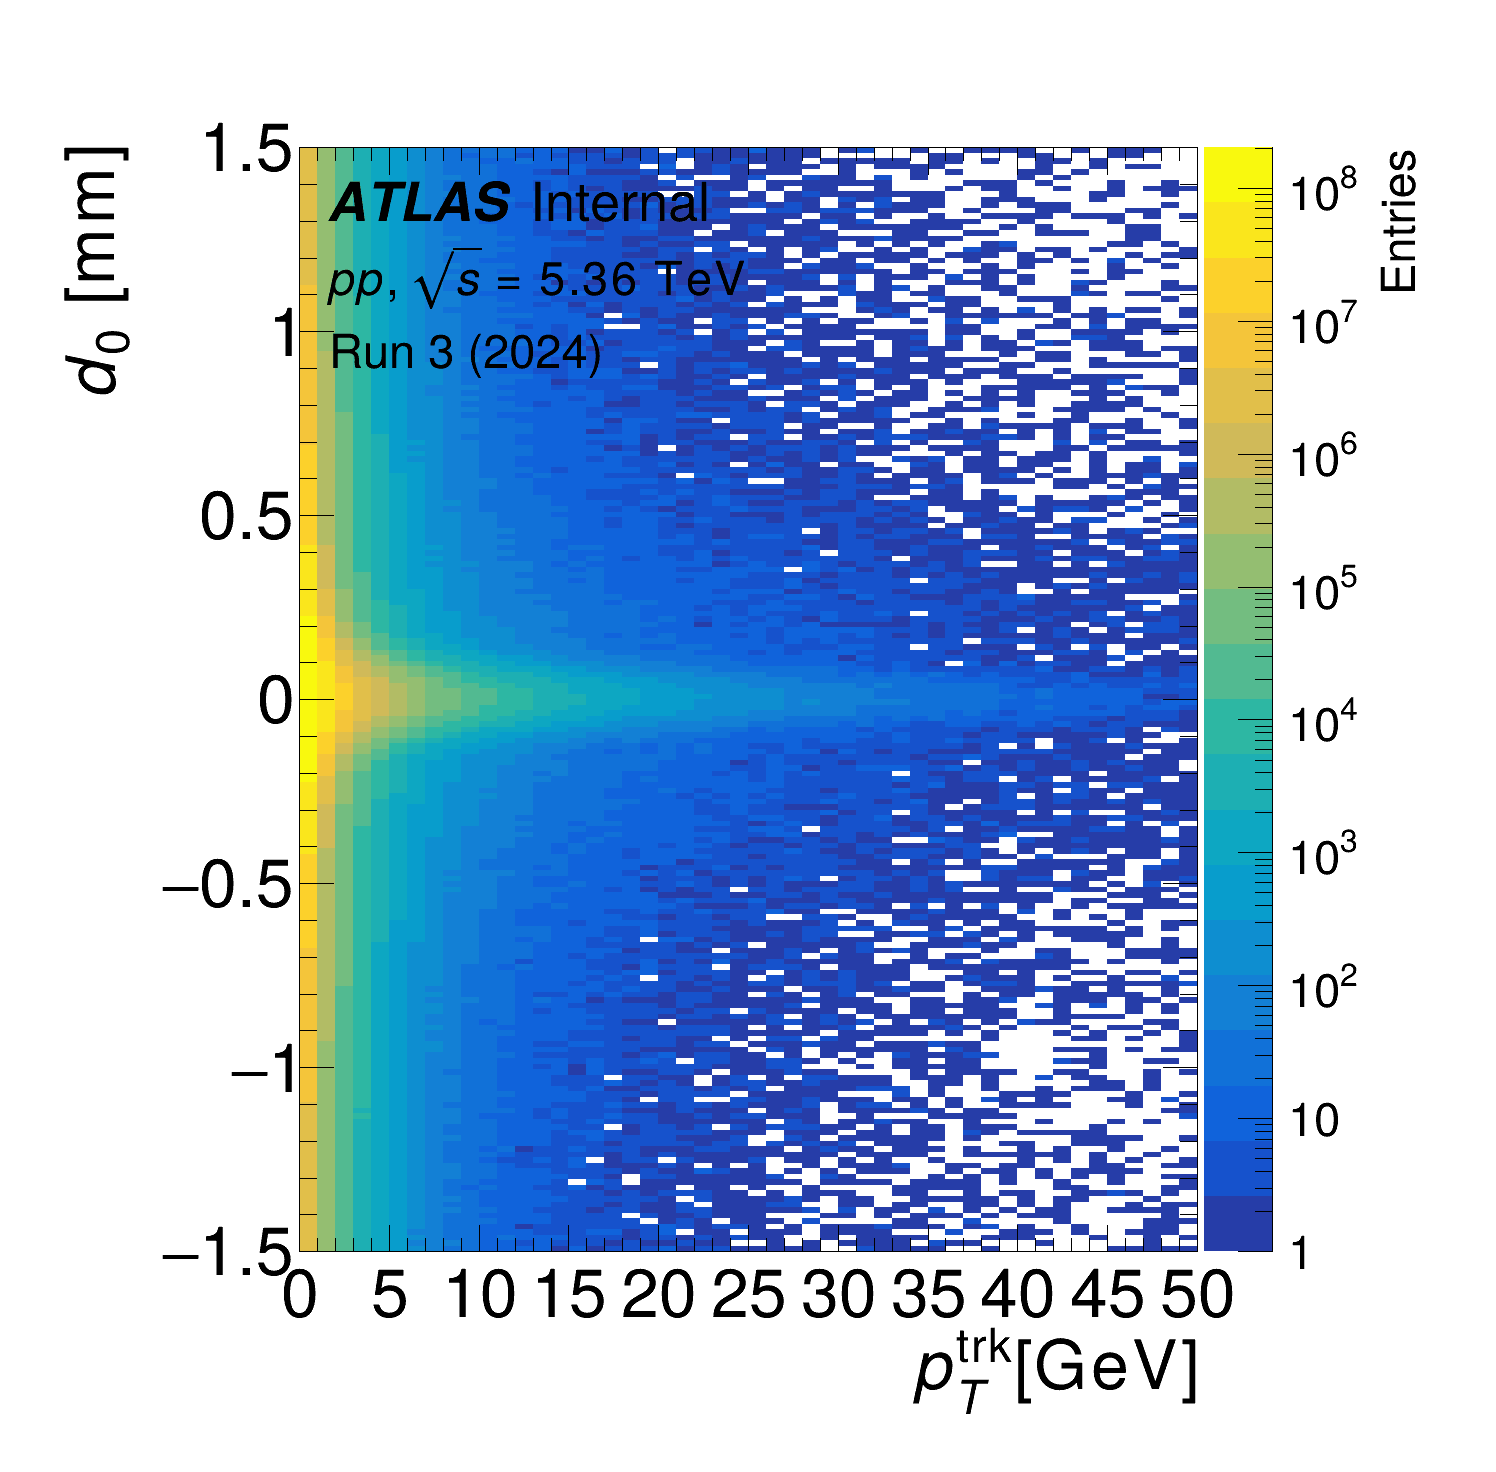
\includegraphics[width=0.32\linewidth]{images/d0_vs_pt_almost_all_h2d_d0_vs_pt_cut0_.png}
    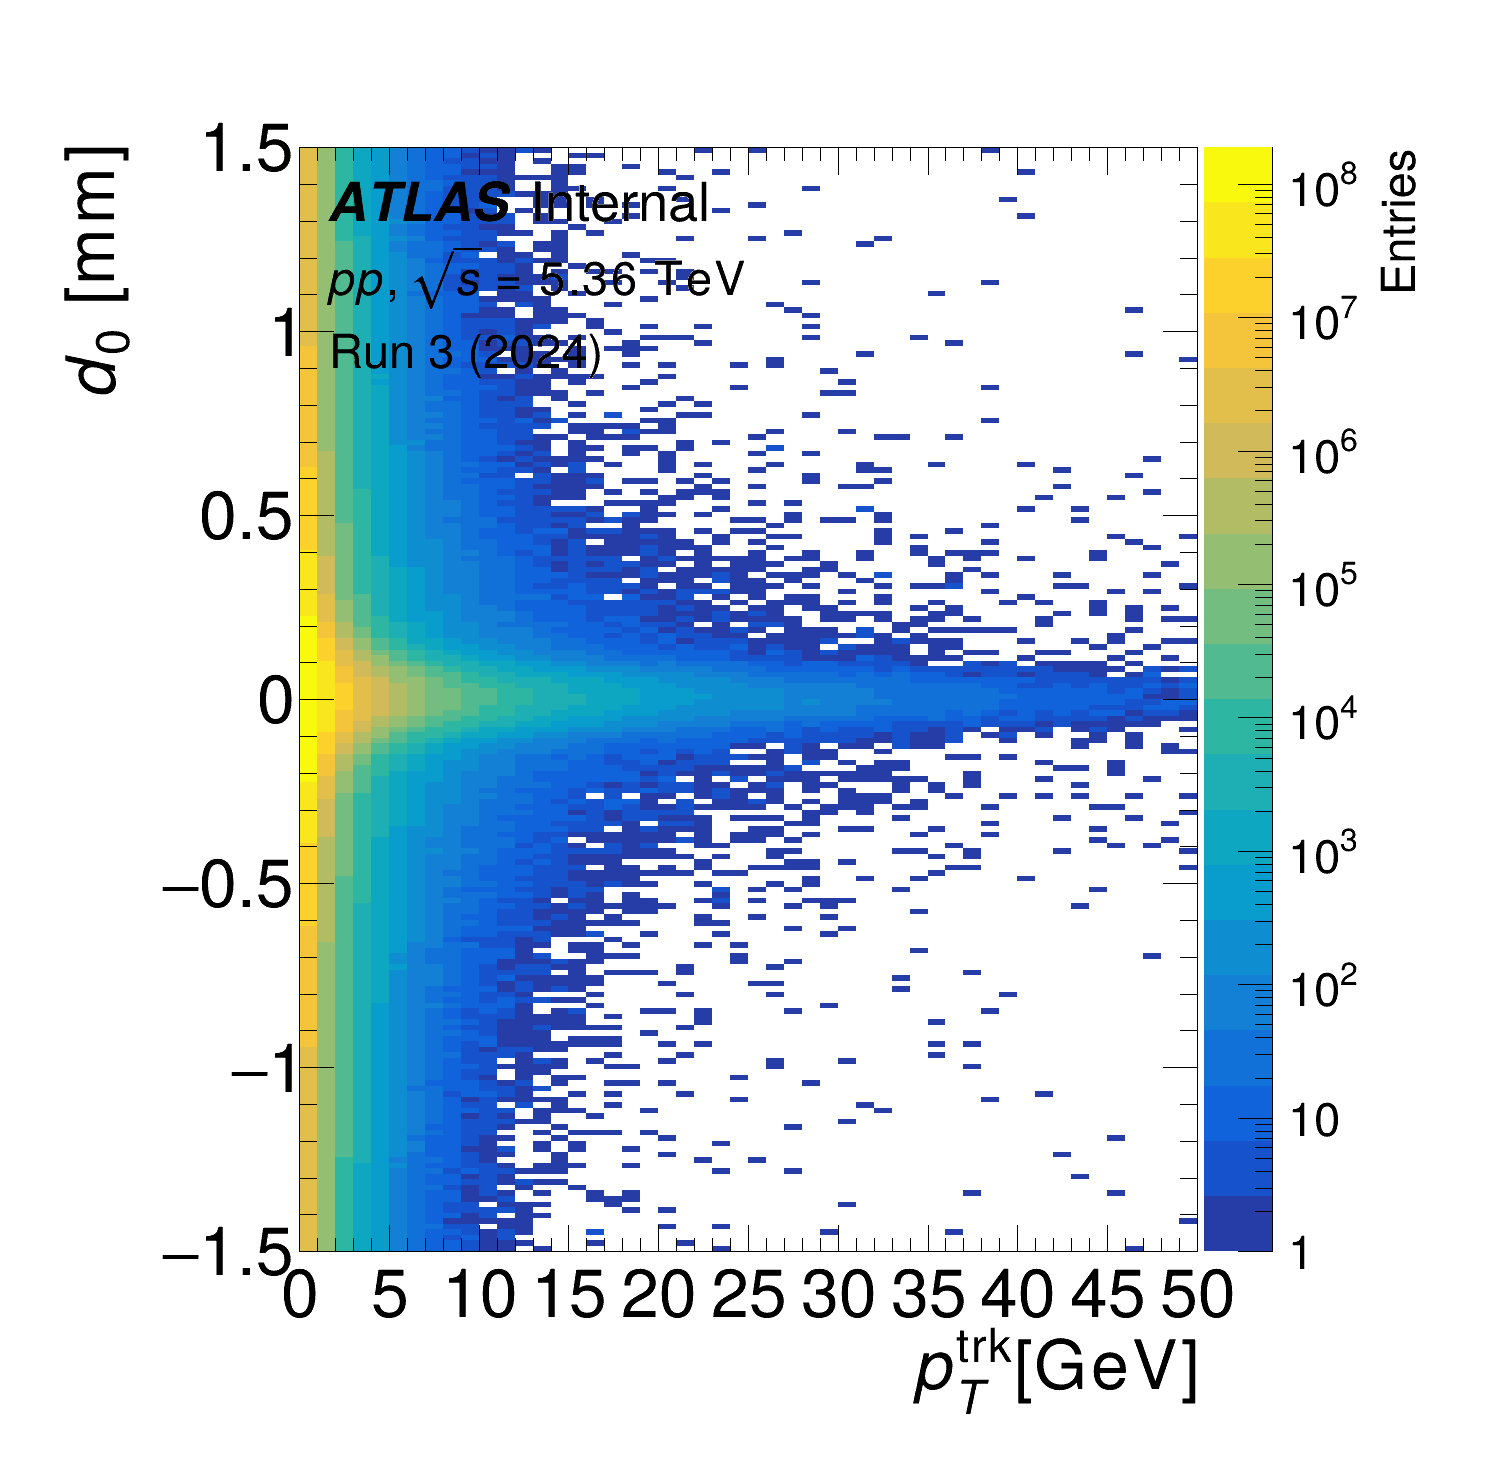
\includegraphics[width=0.32\linewidth]{images/d0_vs_pt_almost_all_h2d_d0_vs_pt_cut1_.png}
    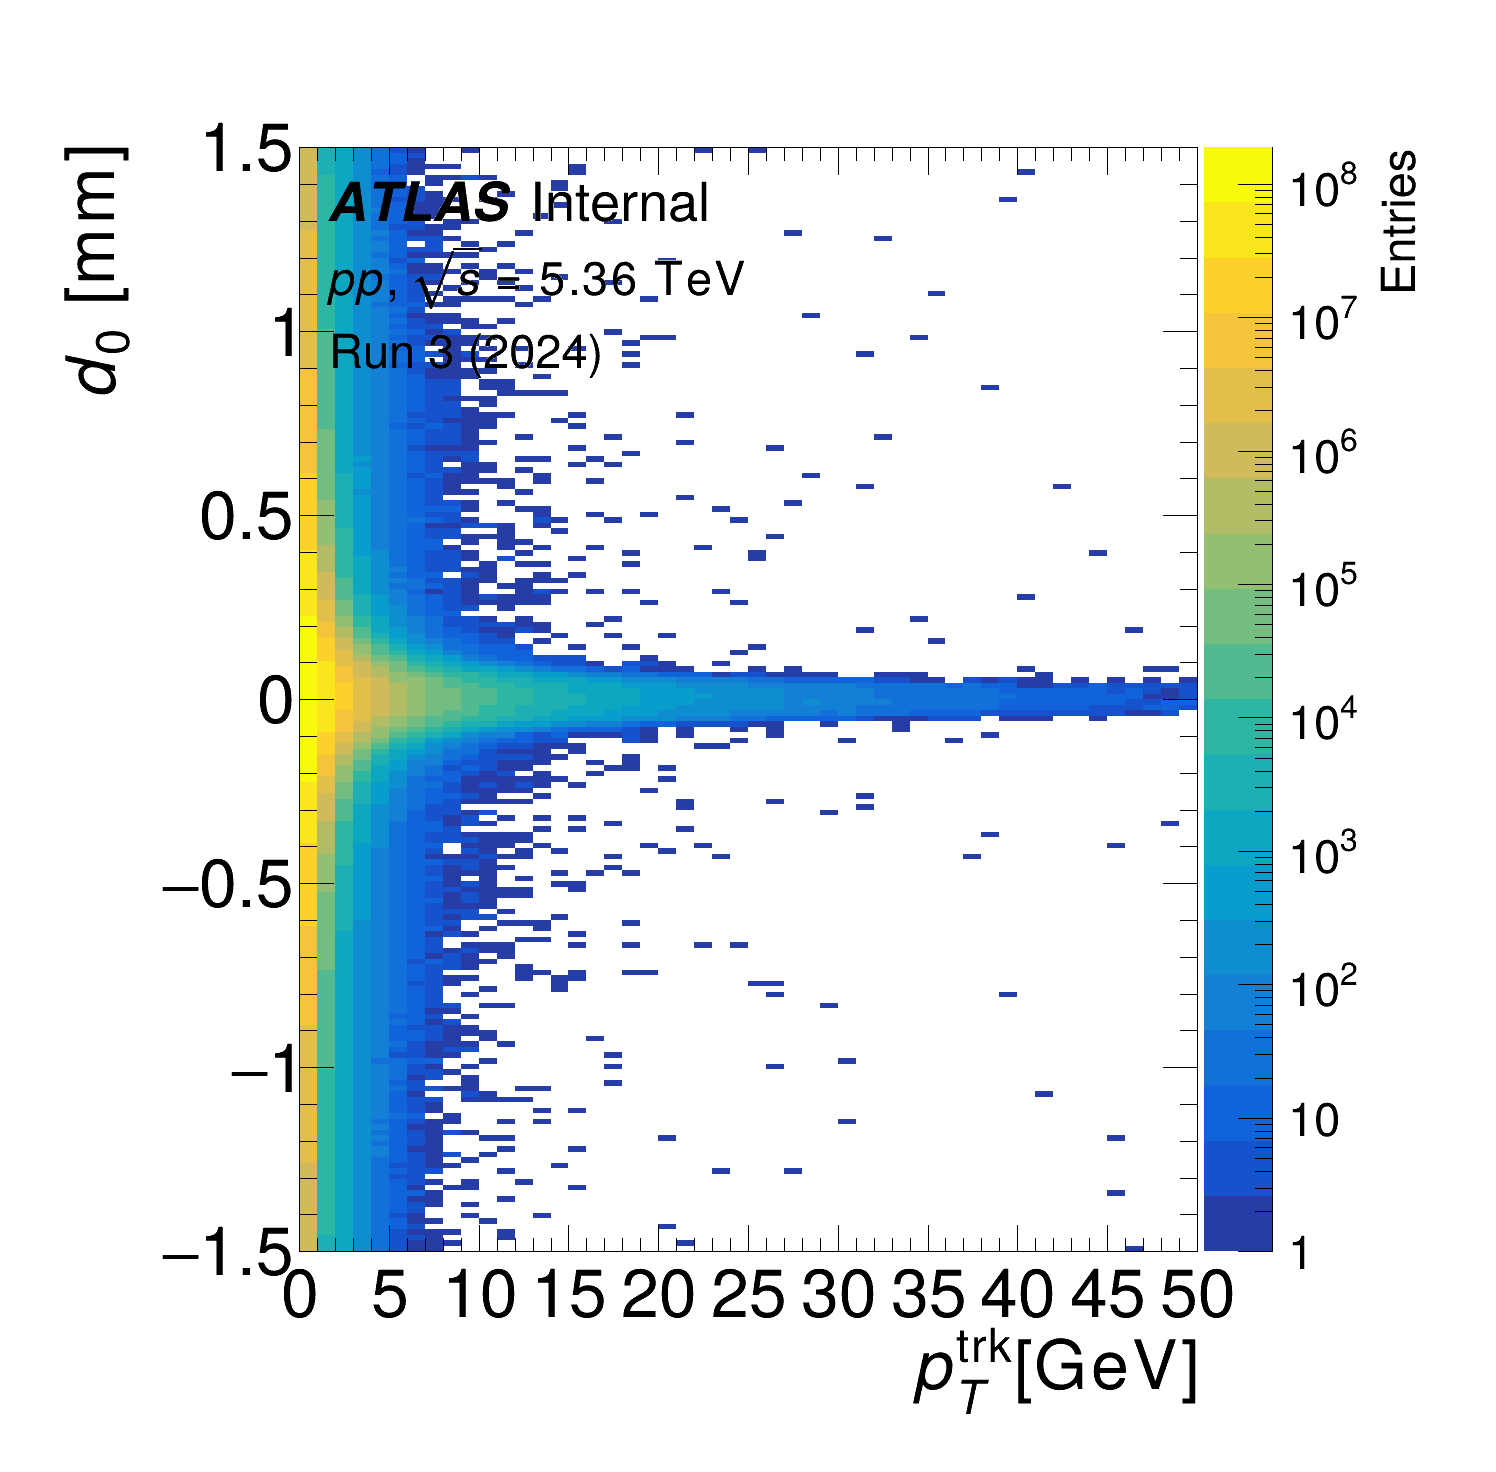
\includegraphics[width=0.32\linewidth]{images/d0_vs_pt_almost_all_h2d_d0_vs_pt_cut3_.png}
    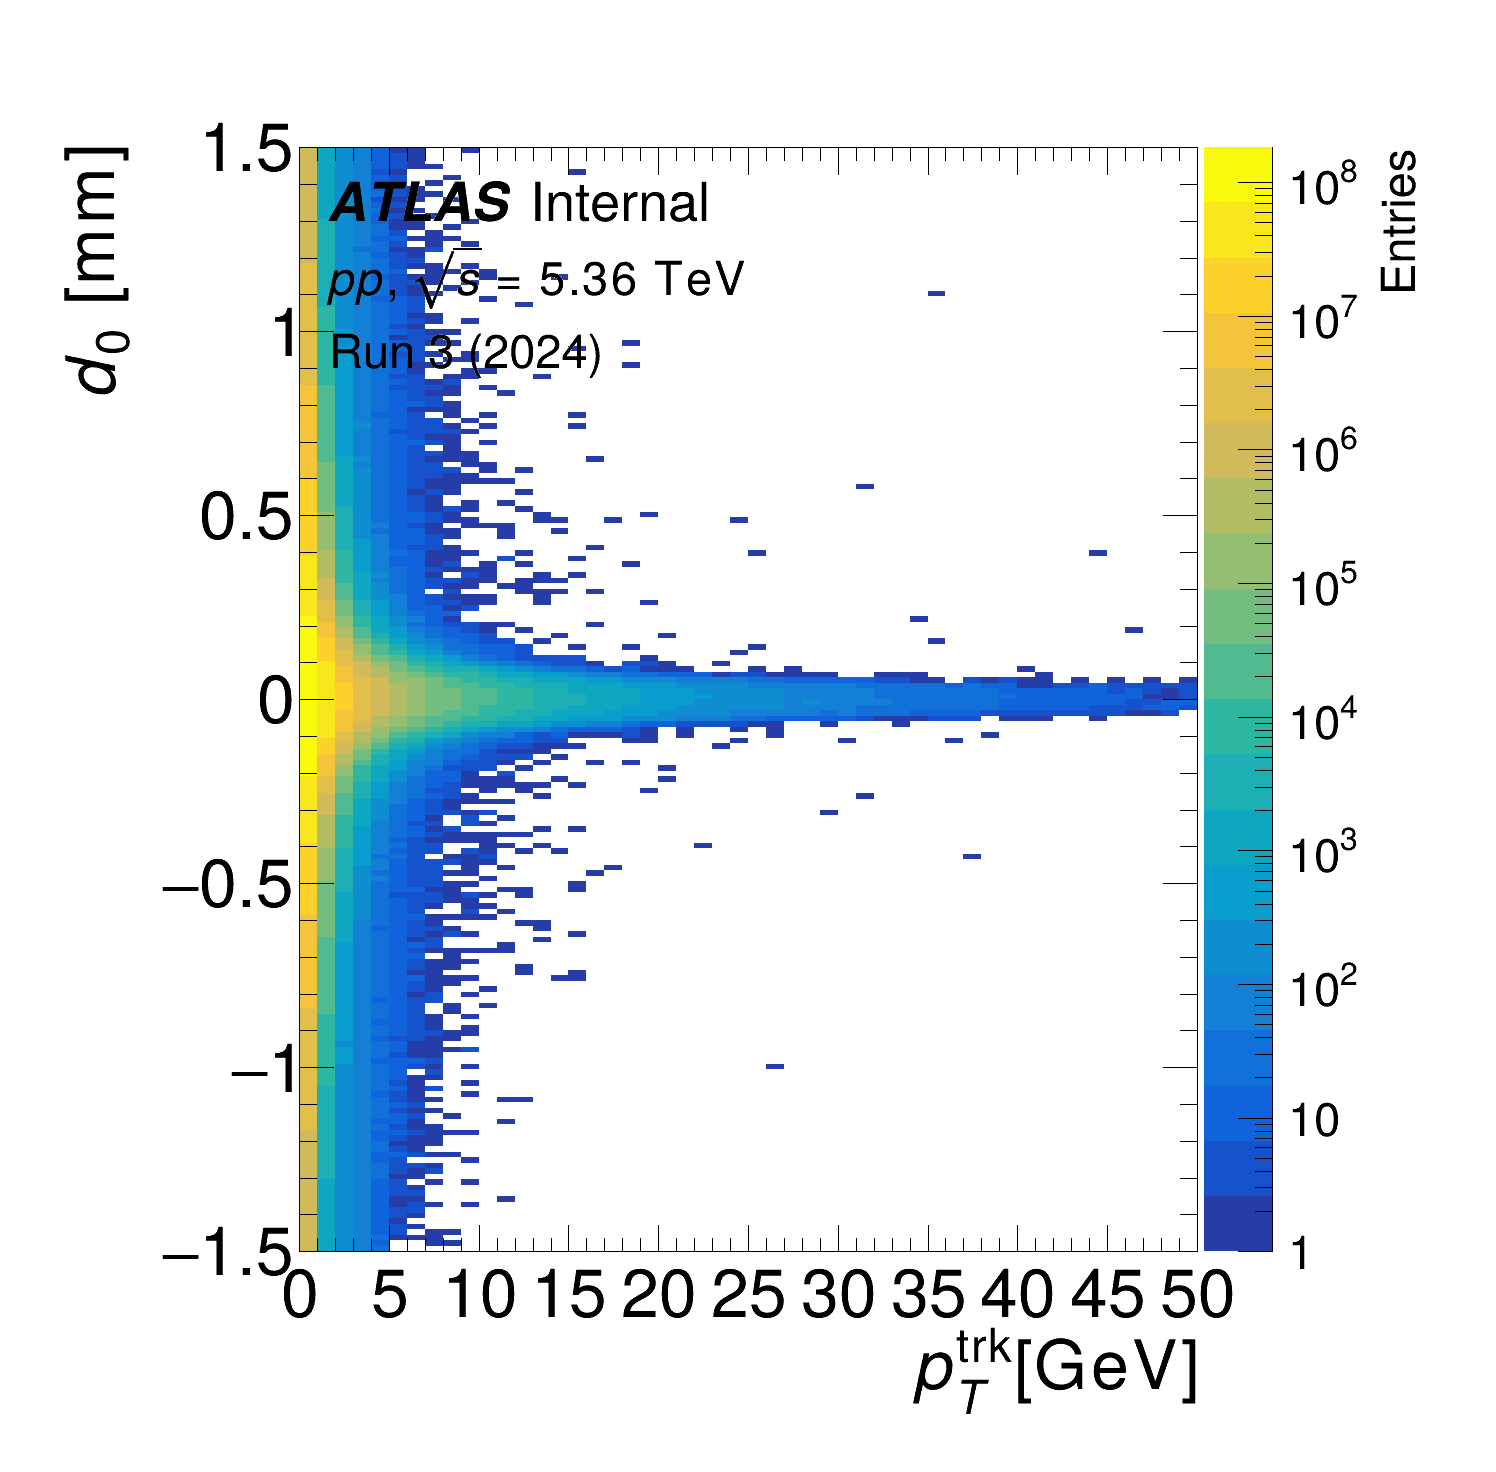
\includegraphics[width=0.32\linewidth]{images/d0_vs_pt_almost_all_h2d_d0_vs_pt_cut4_.png}
    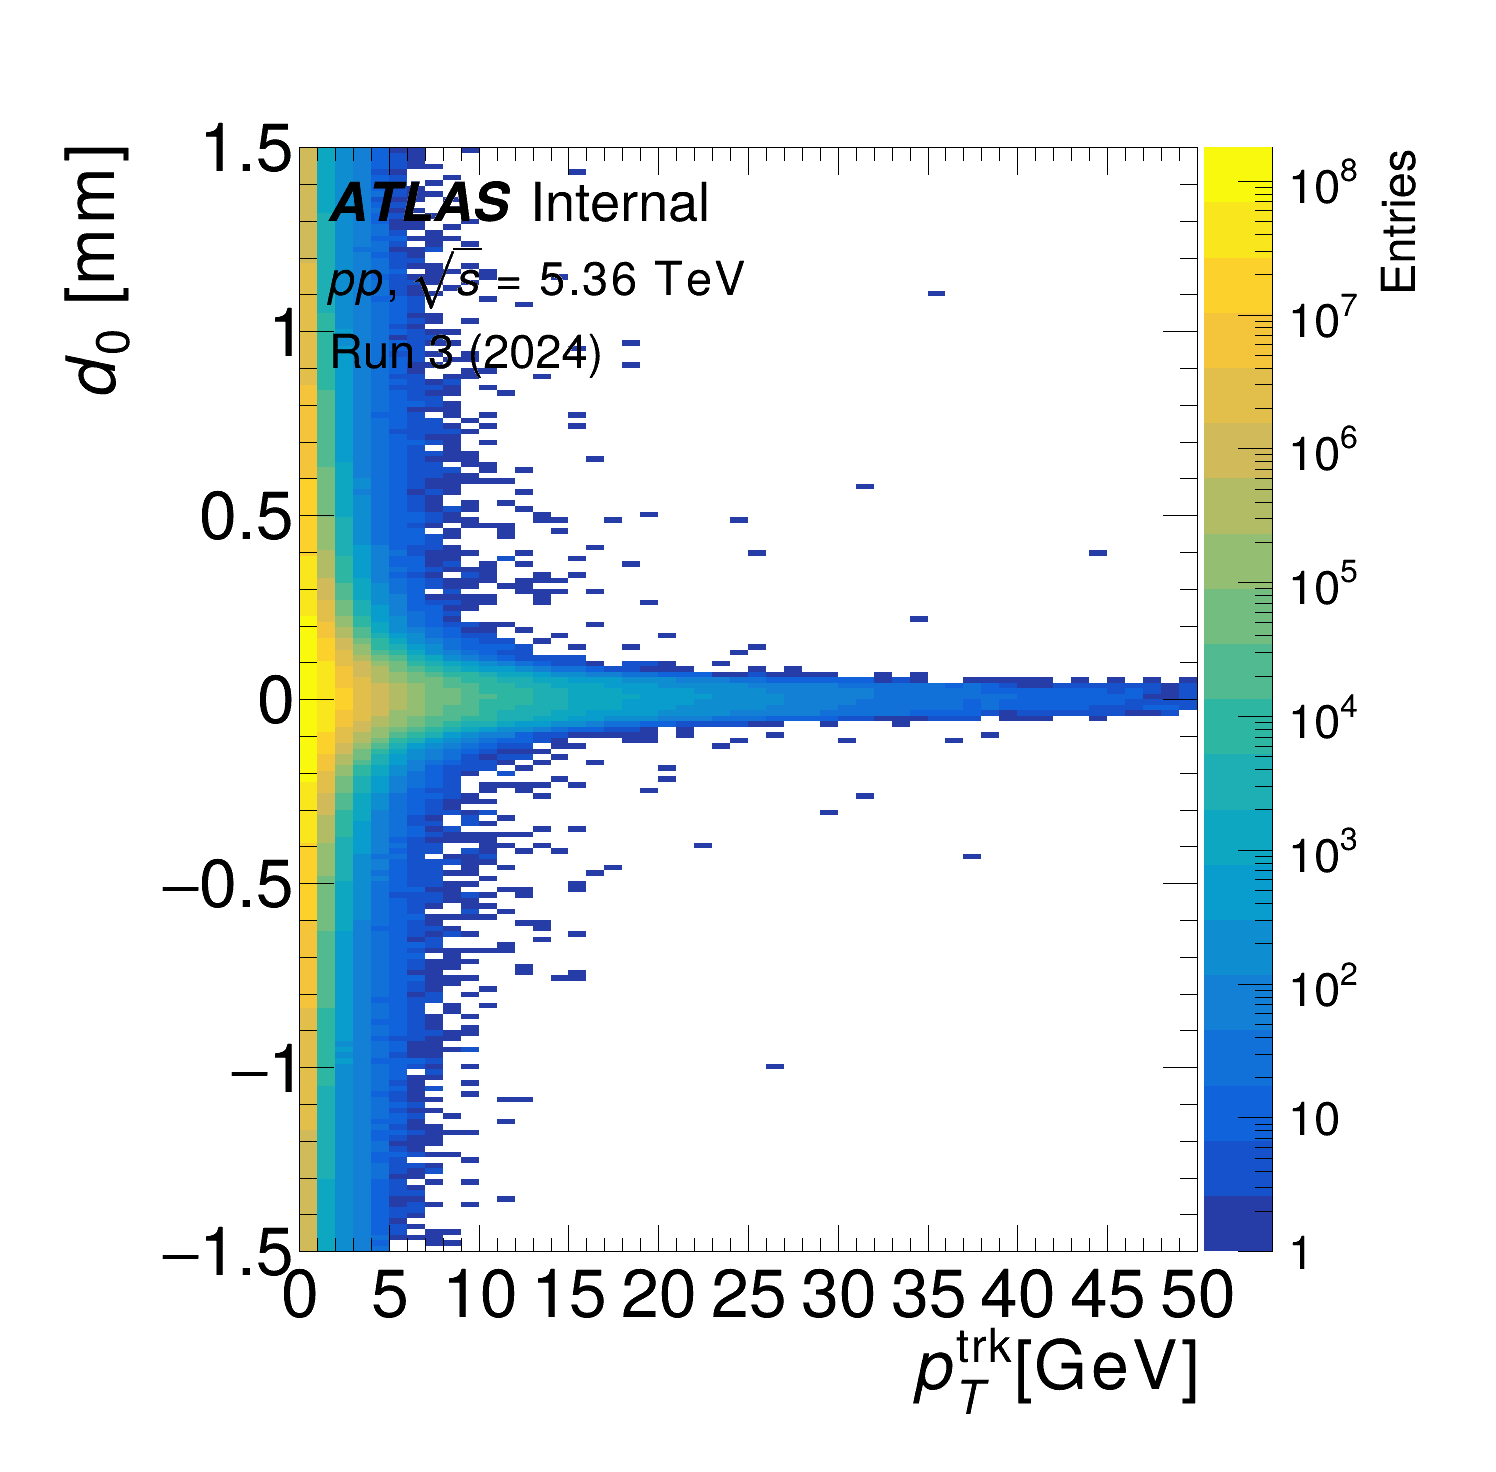
\includegraphics[width=0.32\linewidth]{images/d0_vs_pt_almost_all_h2d_d0_vs_pt_cut5_.png}
    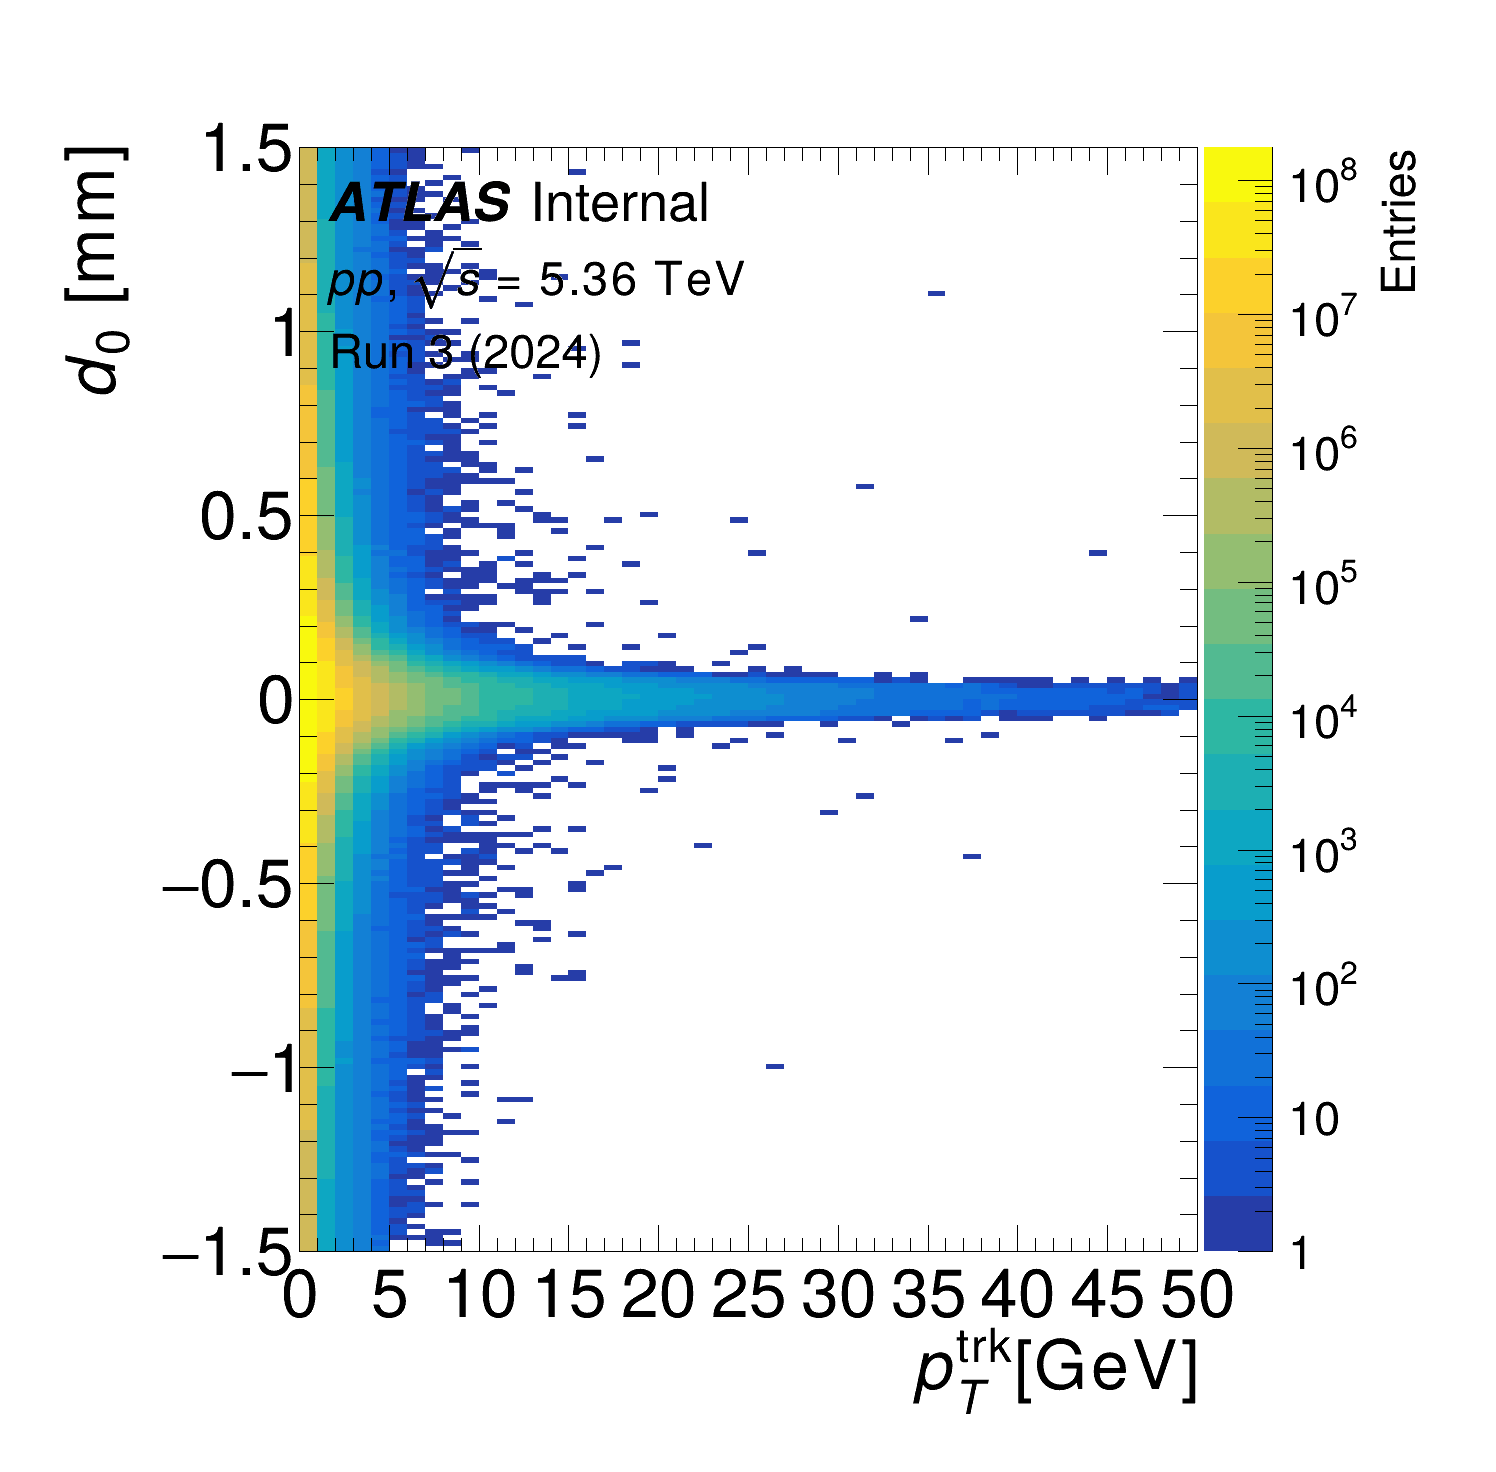
\includegraphics[width=0.32\linewidth]{images/d0_vs_pt_almost_all_h2d_d0_vs_pt_cut6_.png}
    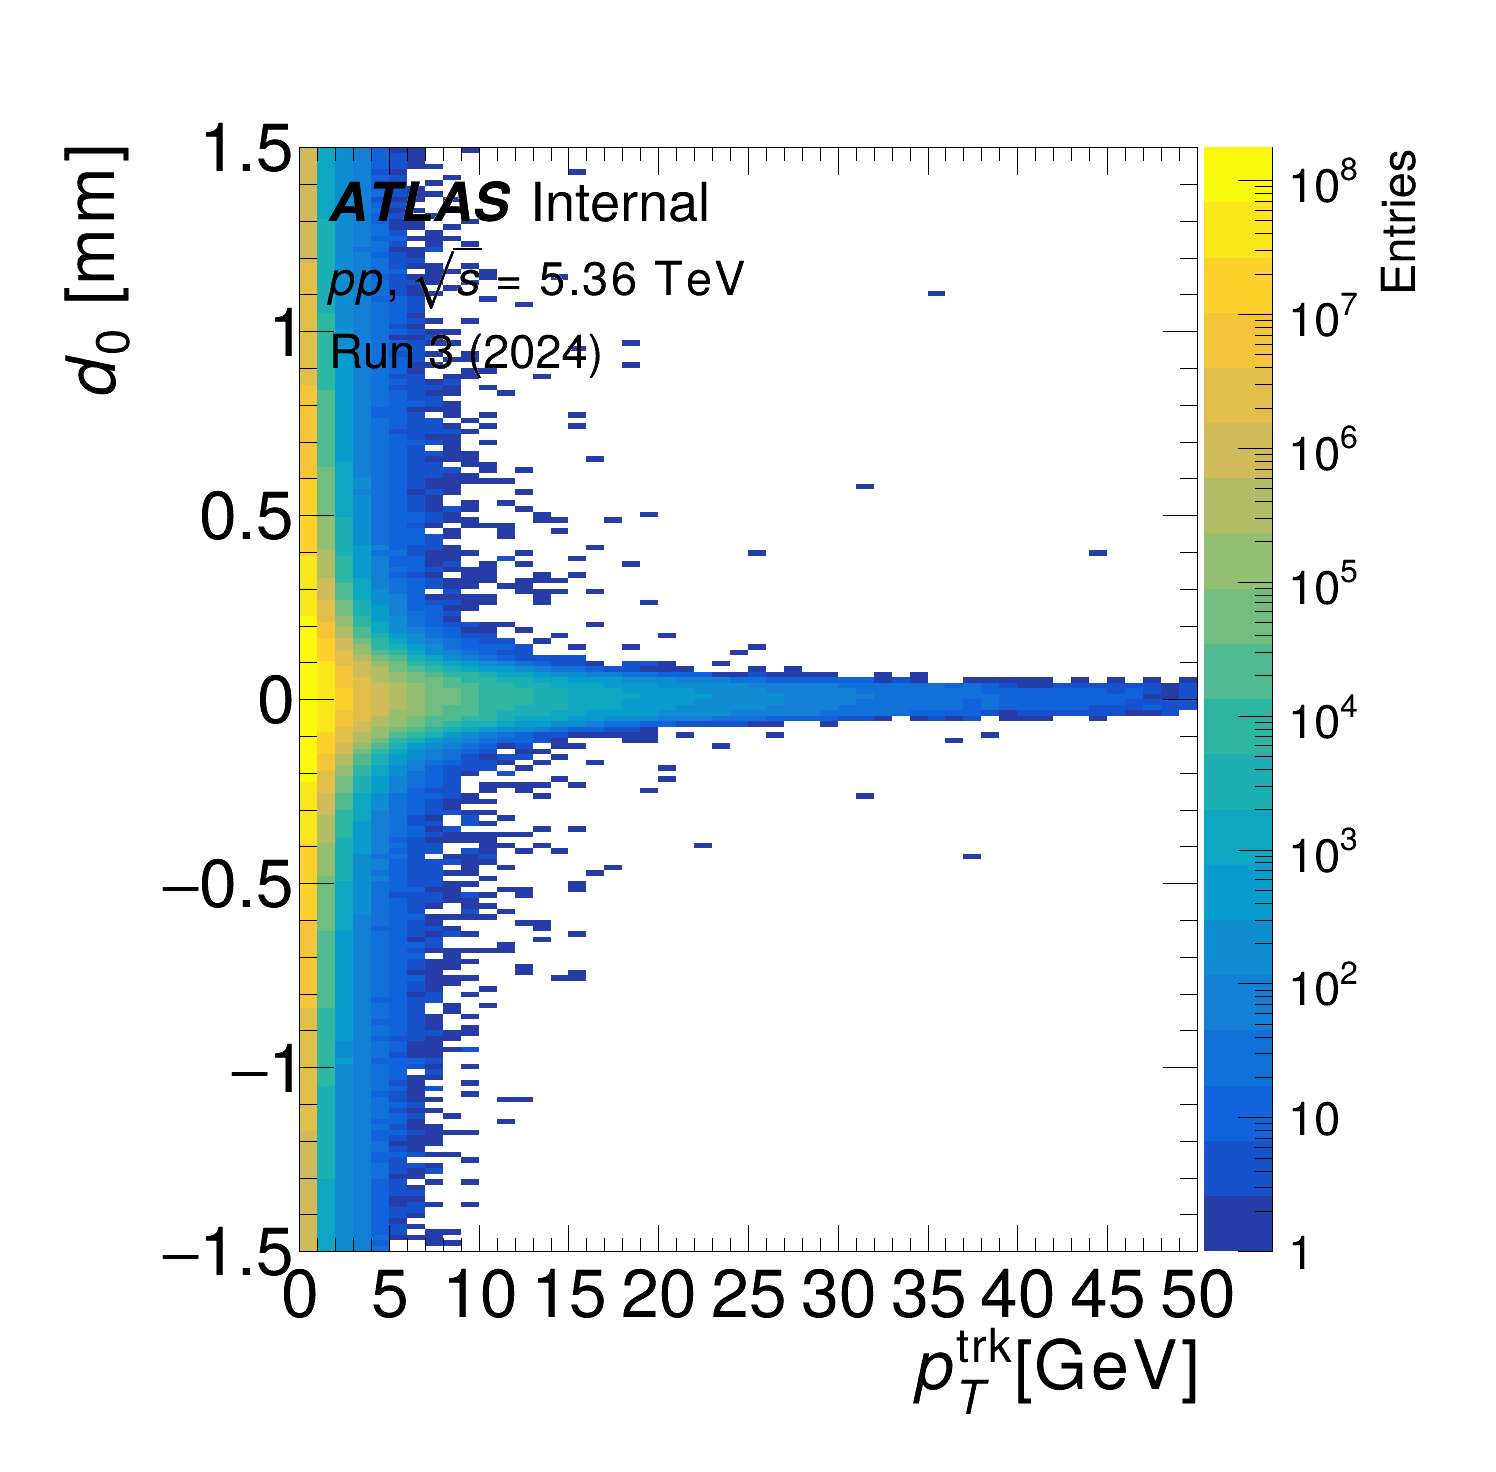
\includegraphics[width=0.32\linewidth]{images/d0_vs_pt_almost_all_h2d_d0_vs_pt_cut7_.png}
    %\caption{Left: tracks with "Loose" quality. Middle: "TightPrimary" and $|d_0|<\qty{1.5}{\mm}$, $|d_0/\sigma_{d_0}| < 4$. Right: Additionally requiring $|\omega_0|<\qty{1.5}{\mm}$ and $|\omega_0/\sigma_{\omega_0}| < 4$}
    \caption{Cutflow of the $d_0$ vs $\pT$. Top row: tracks with "TightPrimary" (left), $|d_0|<\qty{1.5}{\mm}$  and $|d_0/\sigma_{d_0}| < 4$ (middle), $|\omega_0|<\qty{1.5}{\mm}$ (right). Bottom row: $|\omega_0/\sigma_{\omega_0}| < 4$ (left), $|z_\text{vtx}|<150$ mm (middle), jet-matched (right, see text)}
    \label{fig:cutflow_d0}
\end{figure}

Next, the track-to-vertex matching in $z$ was studied using the following variables defined for each track:
\begin{equation}
    \Delta z_0 = \pm\min_{i} |z_0 + v_z - z_{\text{vtx}i}|, \quad \omega_0 = \Delta z_0 \sin\theta,
\end{equation}
where $v_z$ is the reference point of calculation of $z_0$ for a given track, $z_{\text{vtx}i}$ is the position along $z$ of vertex $i$.
Each track is therefore assigned to a vertex $\text{vtx}_i$, based on the distance in $z$. Next, the given track is matched to its assigned vertex if 
\begin{equation}
    |\omega_0| < \qty{1.5}{\mm}, \quad |\omega_0/\sigma_{\omega_0}| < 4,
\end{equation}
where $\sigma_{\omega_0}$ is the standard error of $\omega_0$, which is inferred from errors on $z_0$ and $\theta$ as 
\begin{equation}
    \sigma_{\omega_0} = \sqrt{\sigma^2_{z_0}\sin^2\theta + \sigma^2_{\theta}(\Delta z_0)^2\cos^2\theta}
\end{equation}
The effect of the $|\omega_0|$ cut is demonstrated on Figure~\ref{fig:cutflow_d0}. Such a cut depends on $\mu$ as the number of merged vertices rises with $\mu$ \cite{ATLAS:2016nnj}. If two vertices merge into one, $z$ of both of them moves towards the center of mass of the pair. Consequently, the associated tracks will have greater $\omega_0$, which can be seen on the right plot of Figure~\ref{fig:lowmu_highmu_ip_norm}. The effect of merging in a perpendicular plane to the beamline is not very strong (see Figure~\ref{fig:lowmu_highmu_ip_norm}, left), because the ''effective area'' is much smaller (see sec.~\ref{sec:vertex_merging}). 
\begin{figure}[h]
    \centering
    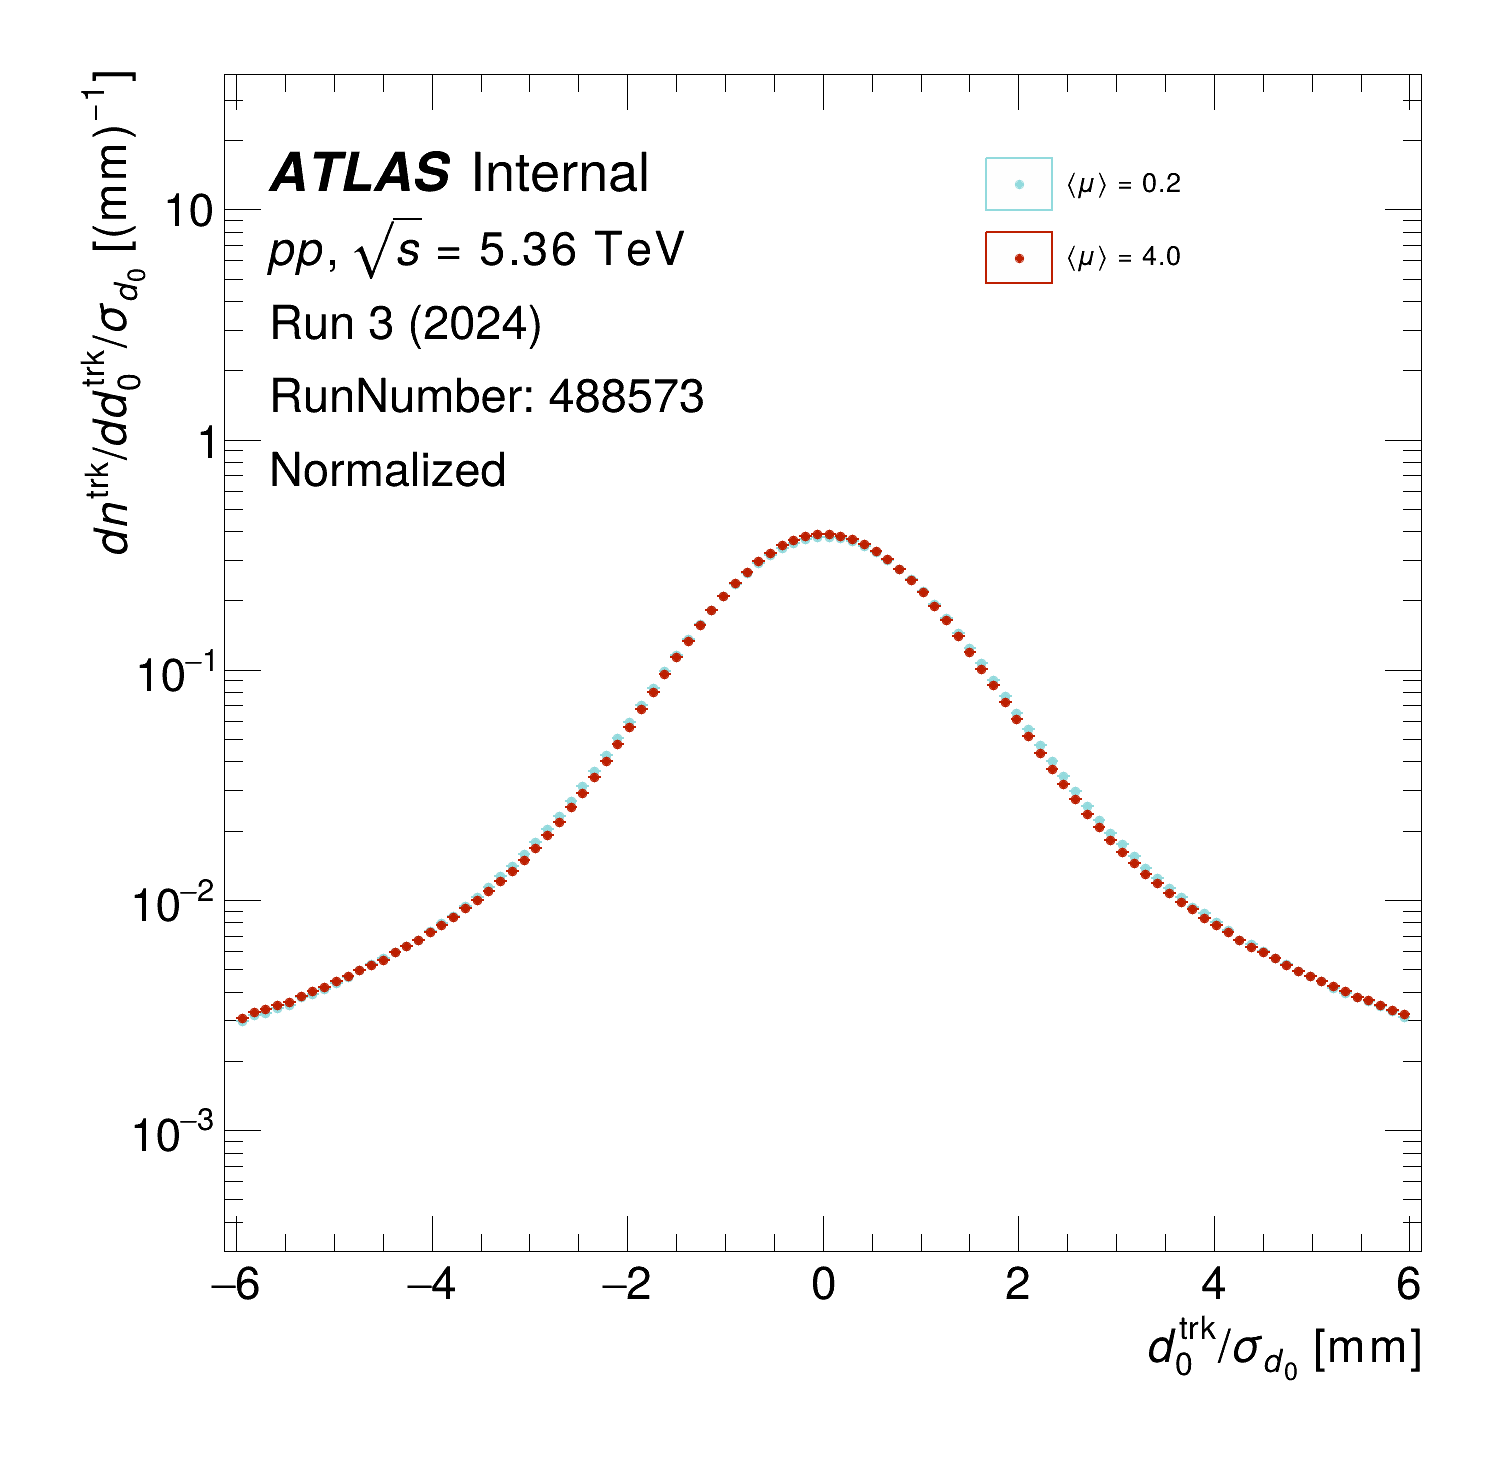
\includegraphics[width=0.49\linewidth]{images/trk_d0_norm_488573.png}
    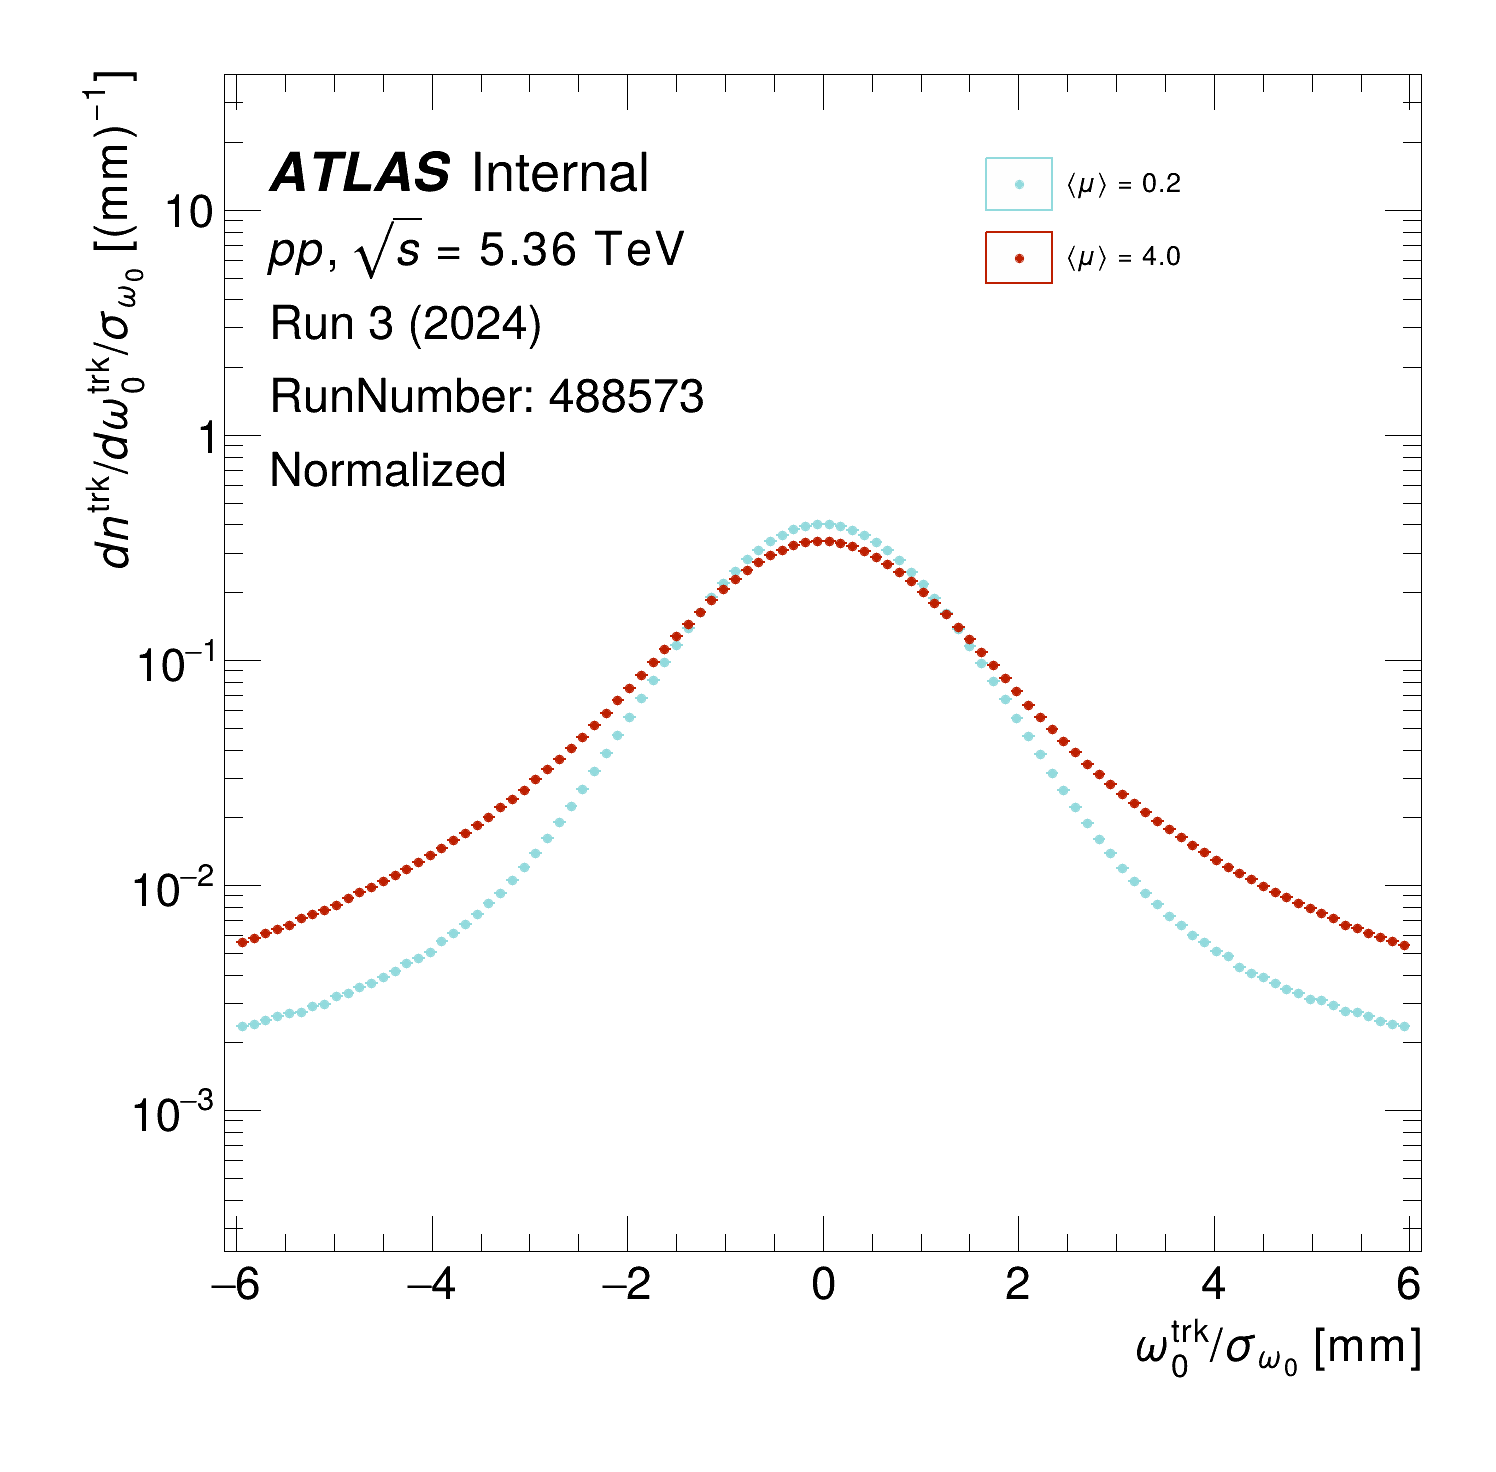
\includegraphics[width=0.49\linewidth]{images/trk_omega0_norm_488573.png}
    \caption{Comparison of track distributions for low-$\mu$ and high-$\mu$ $\pprefSample$ data samples. Left: $d_0/\sigma_{d_0}$ distributions. Right: $\omega_0/\sigma_{\omega_0}$ distributions}
    \label{fig:lowmu_highmu_ip_norm}
\end{figure}

{\blue With cuts on $d_0$ and $\omega_0$, tracks are associated with vertices. One can then require tracks to be associated only with vertices within the window of $|z_\text{vtx}|<\qty{150}{\mm}$. Cut on $\omega_0$ implicitly assumes $\nvtx \geq 1$.}

%let's keep an issue of the $\omega_0$ matching open for a moment.



%\begin{enumerate}
%    \item This cut seems to kill a lot of tracks, so we might want to abandon it and not perform matching in $z$ at all. 
%    \item What about cut on $|z_\text{vtx}|<\qty{150}{\mm}$? 
%\end{enumerate}
%}

\section{Track-to-jet matching}
High-\pT tracks mostly originate in jets. Therefore, one can employ track-to-jet matching. The present analysis took a simplistic approach, expecting the kinematic reach to be around $50$ GeV. Using a distance between a track $i$ and a jet $j$ in $\eta-\phi$ plane:
\begin{equation}
    \Delta R_{ij} = \sqrt{(\eta^i - \eta^j)^2 + (\phi^i-\phi^j)^2}, \quad \min_j \Delta R_{ij} = dR_i,
\end{equation}
the track $i$ is matched to a jet if $dR_i < 0.4$. Jet collection used is \textit{AntiKt4HIJets}. No selection criteria on jets are required.
\begin{figure}[h]
    \centering
    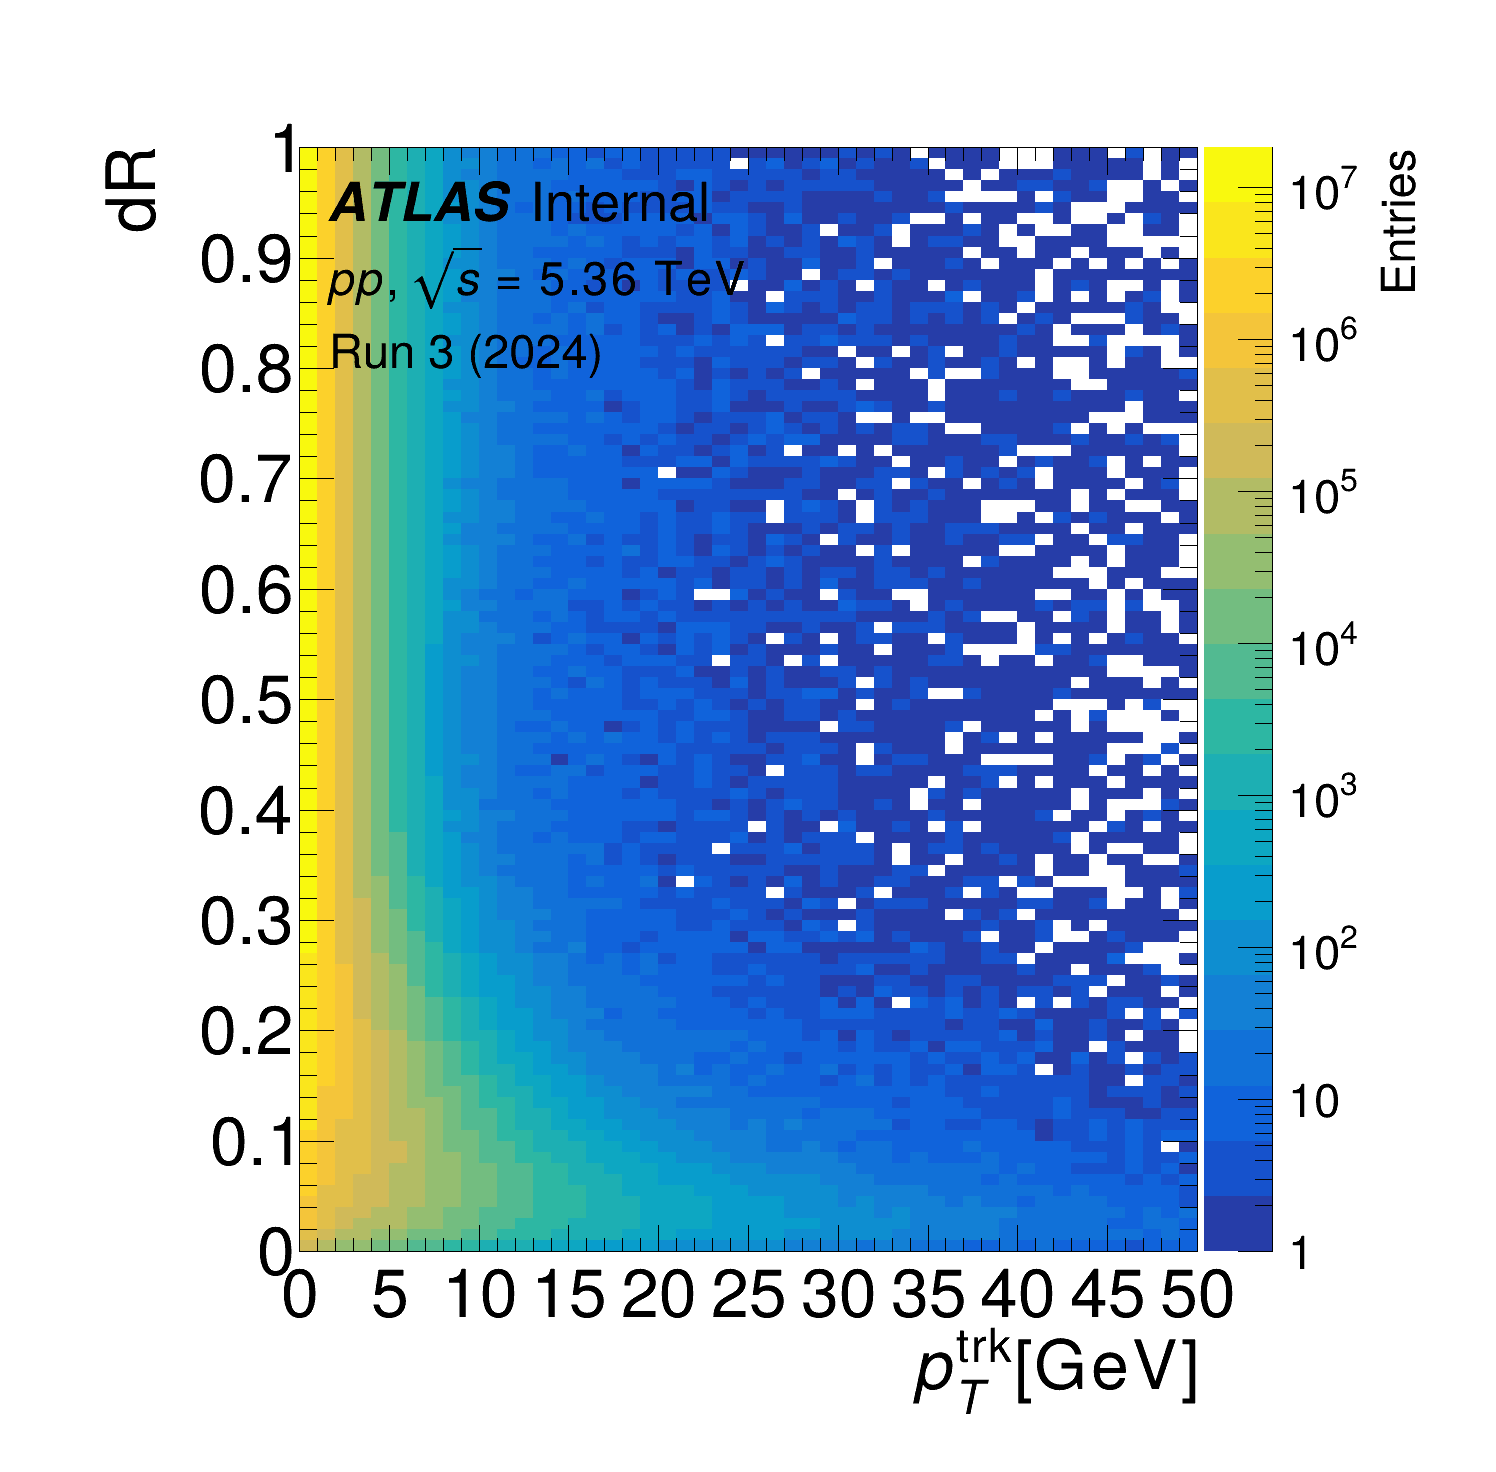
\includegraphics[width=0.32\linewidth]{images/mindR_vs_pt_almost_all_h2d_mindr_vs_pt_cut0_.png}
    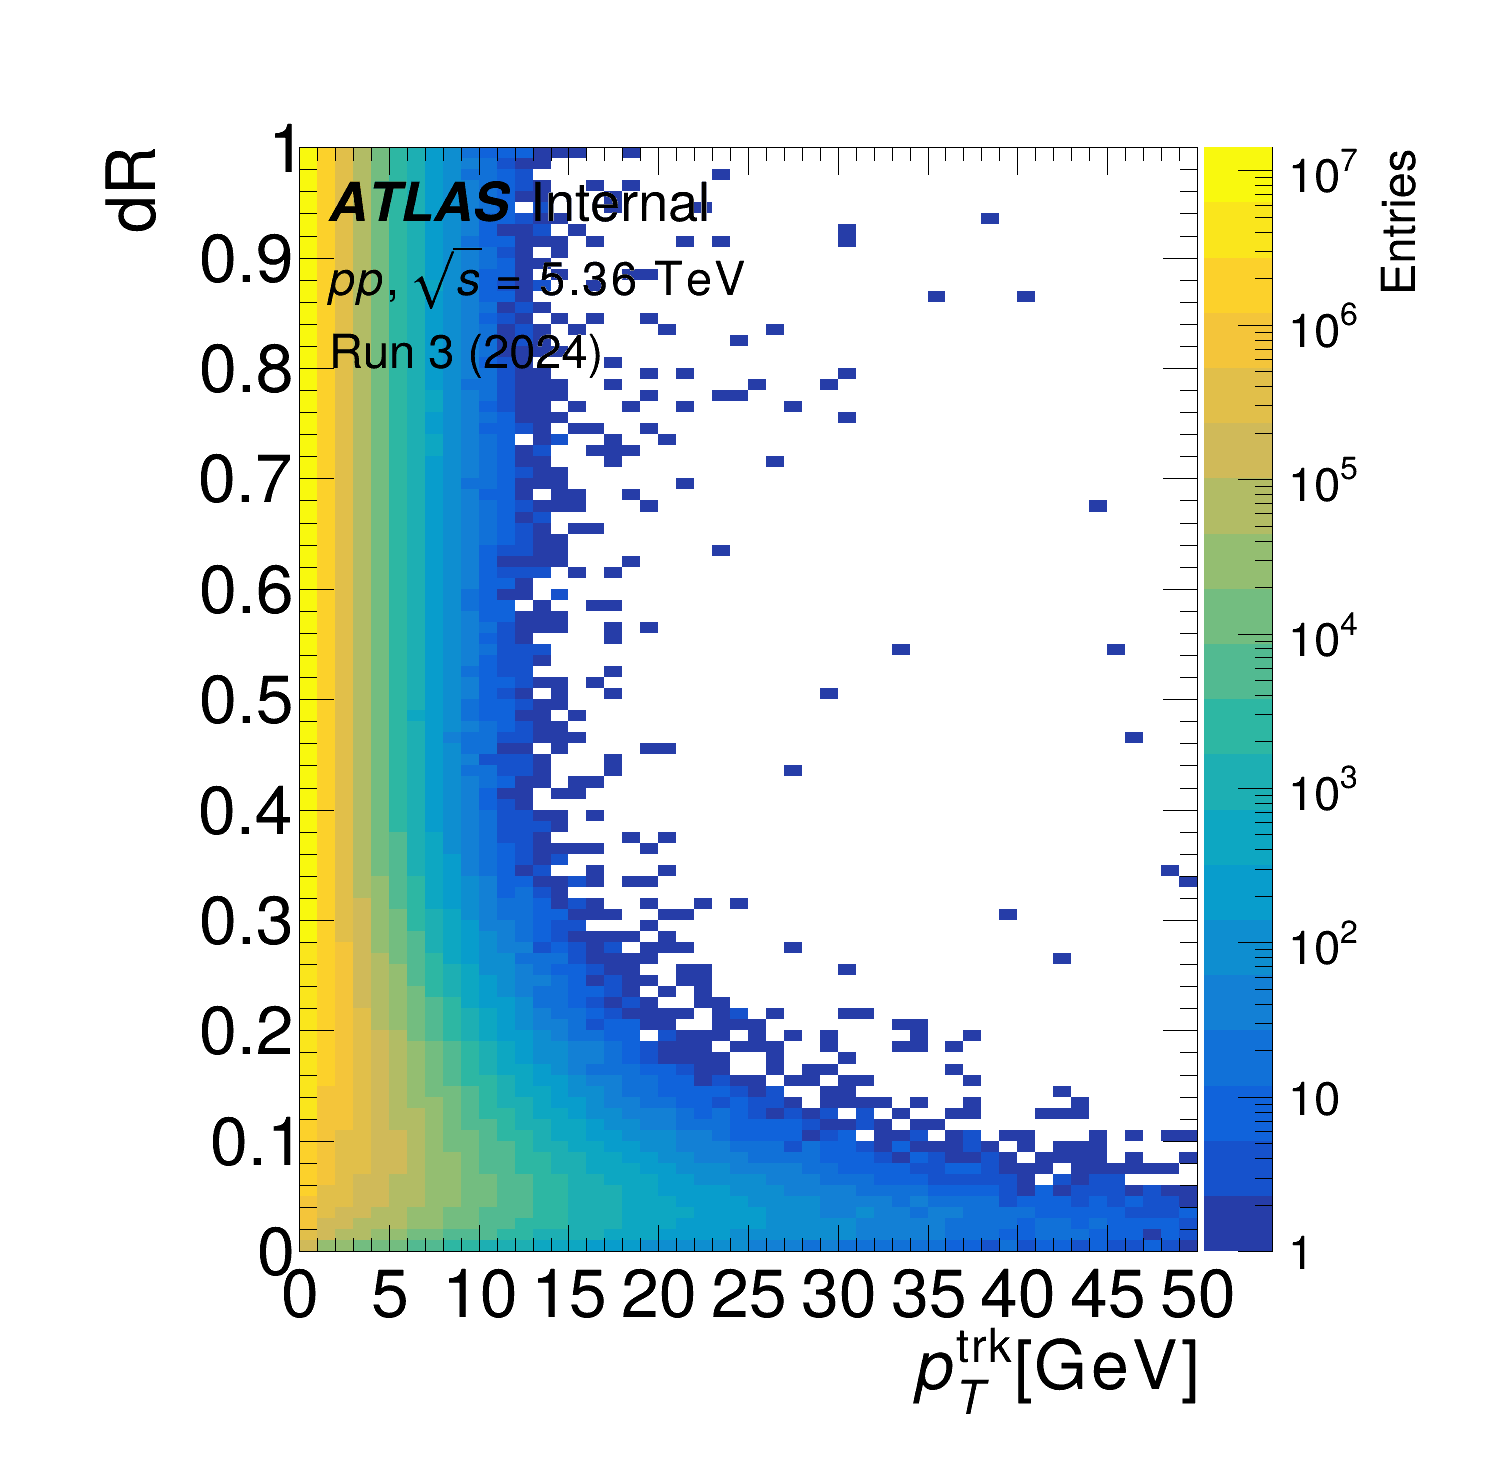
\includegraphics[width=0.32\linewidth]{images/mindR_vs_pt_almost_all_h2d_mindr_vs_pt_cut3_.png}
    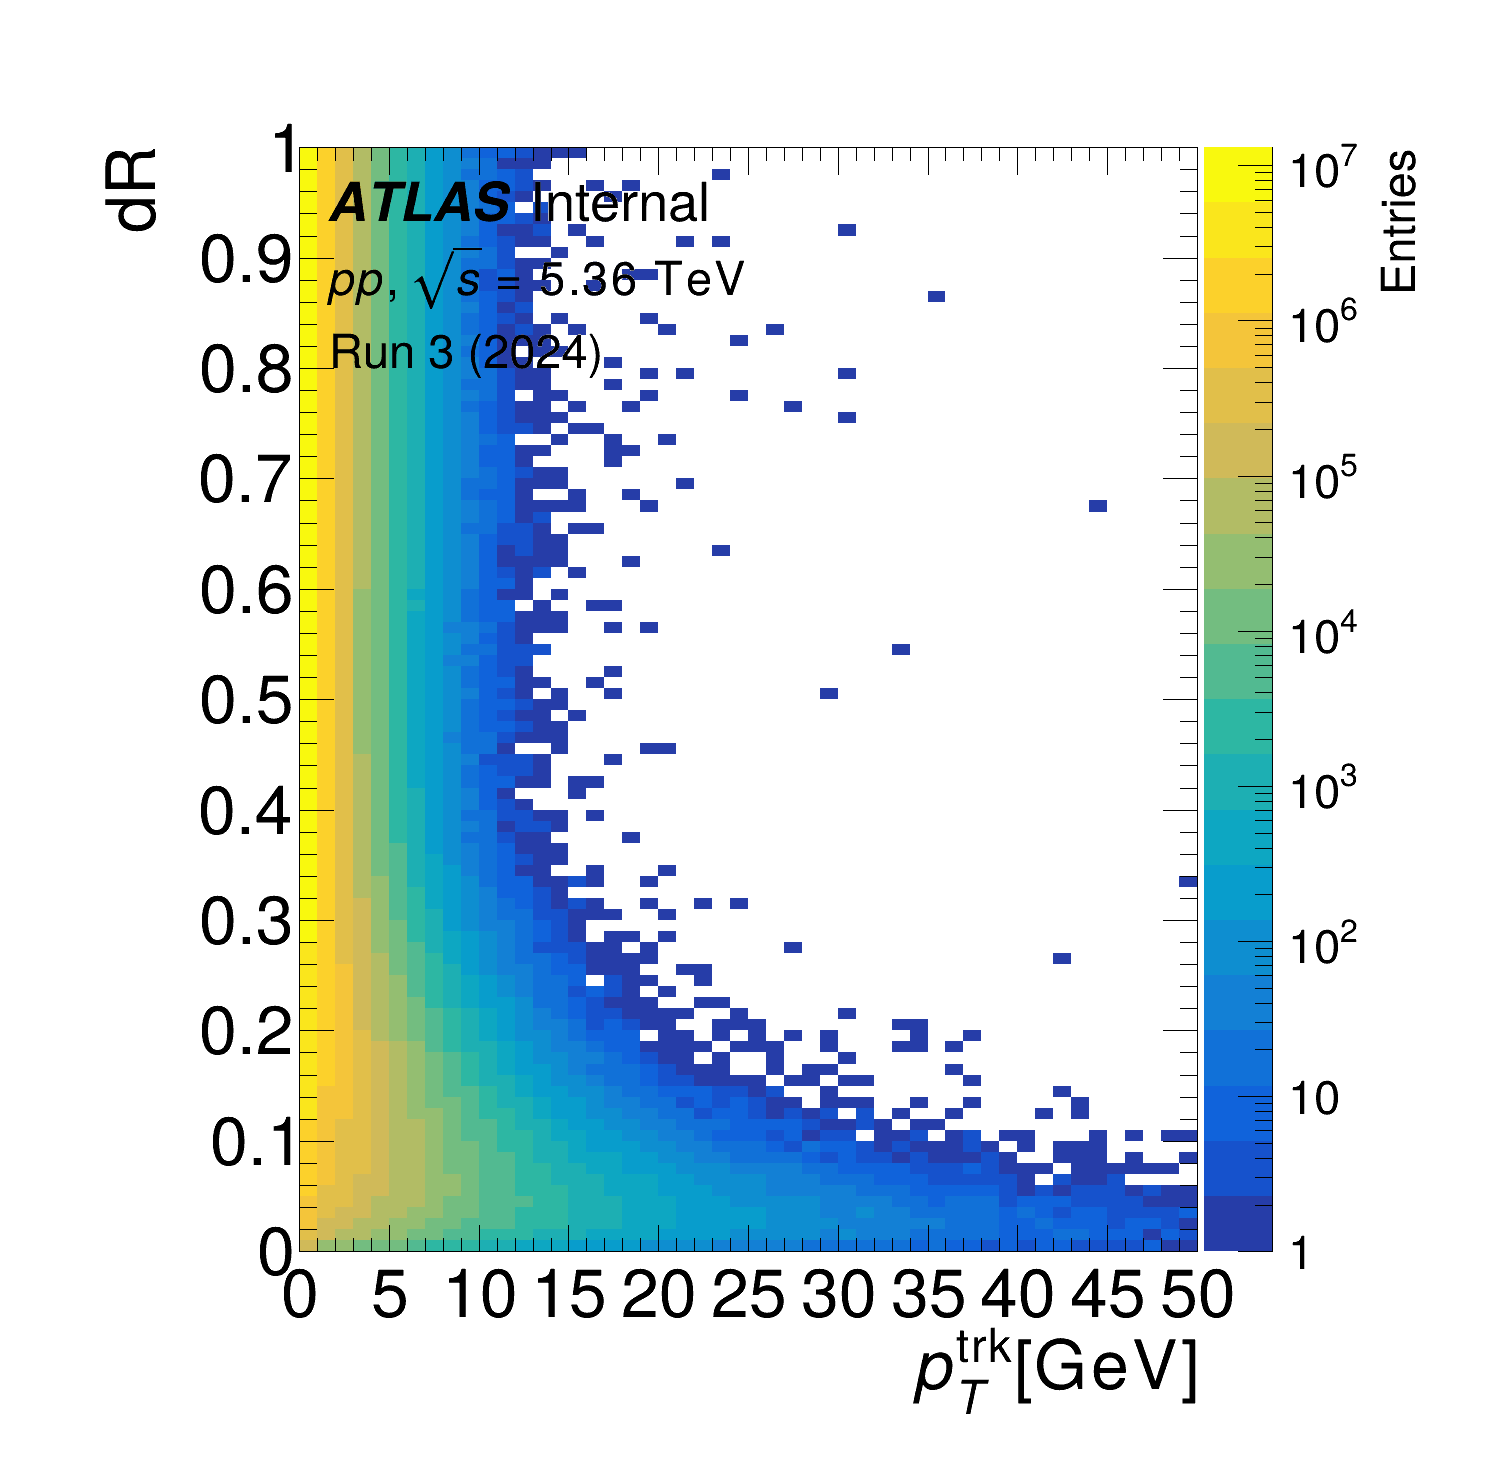
\includegraphics[width=0.32\linewidth]{images/mindR_vs_pt_almost_all_h2d_mindr_vs_pt_cut6_.png}
    \caption{Left: tracks with "Loose" quality. Middle: "TightPrimary" and $|d_0|<\qty{1.5}{\mm}$, $|d_0/\sigma_{d_0}| < 4$. Right: Additionally requiring $|\omega_0|<\qty{1.5}{\mm}$, $|\omega_0/\sigma_{\omega_0}| < 4$ and $|z_\text{vtx}|<\qty{150}{\mm}$}
    \label{fig:cutflow_mindr}
\end{figure}

The jet-matching performance can be seen in Figure~\ref{fig:jetmatched_fractions}, where matching efficiency gets close to 1 around 20 GeV and then for higher $\pT$ starts to drop again, therefore we set the cut to be $dR<0.4$ for tracks with $\pT > \qty{20}{\GeV}$
\begin{figure}[h!]
    \centering
    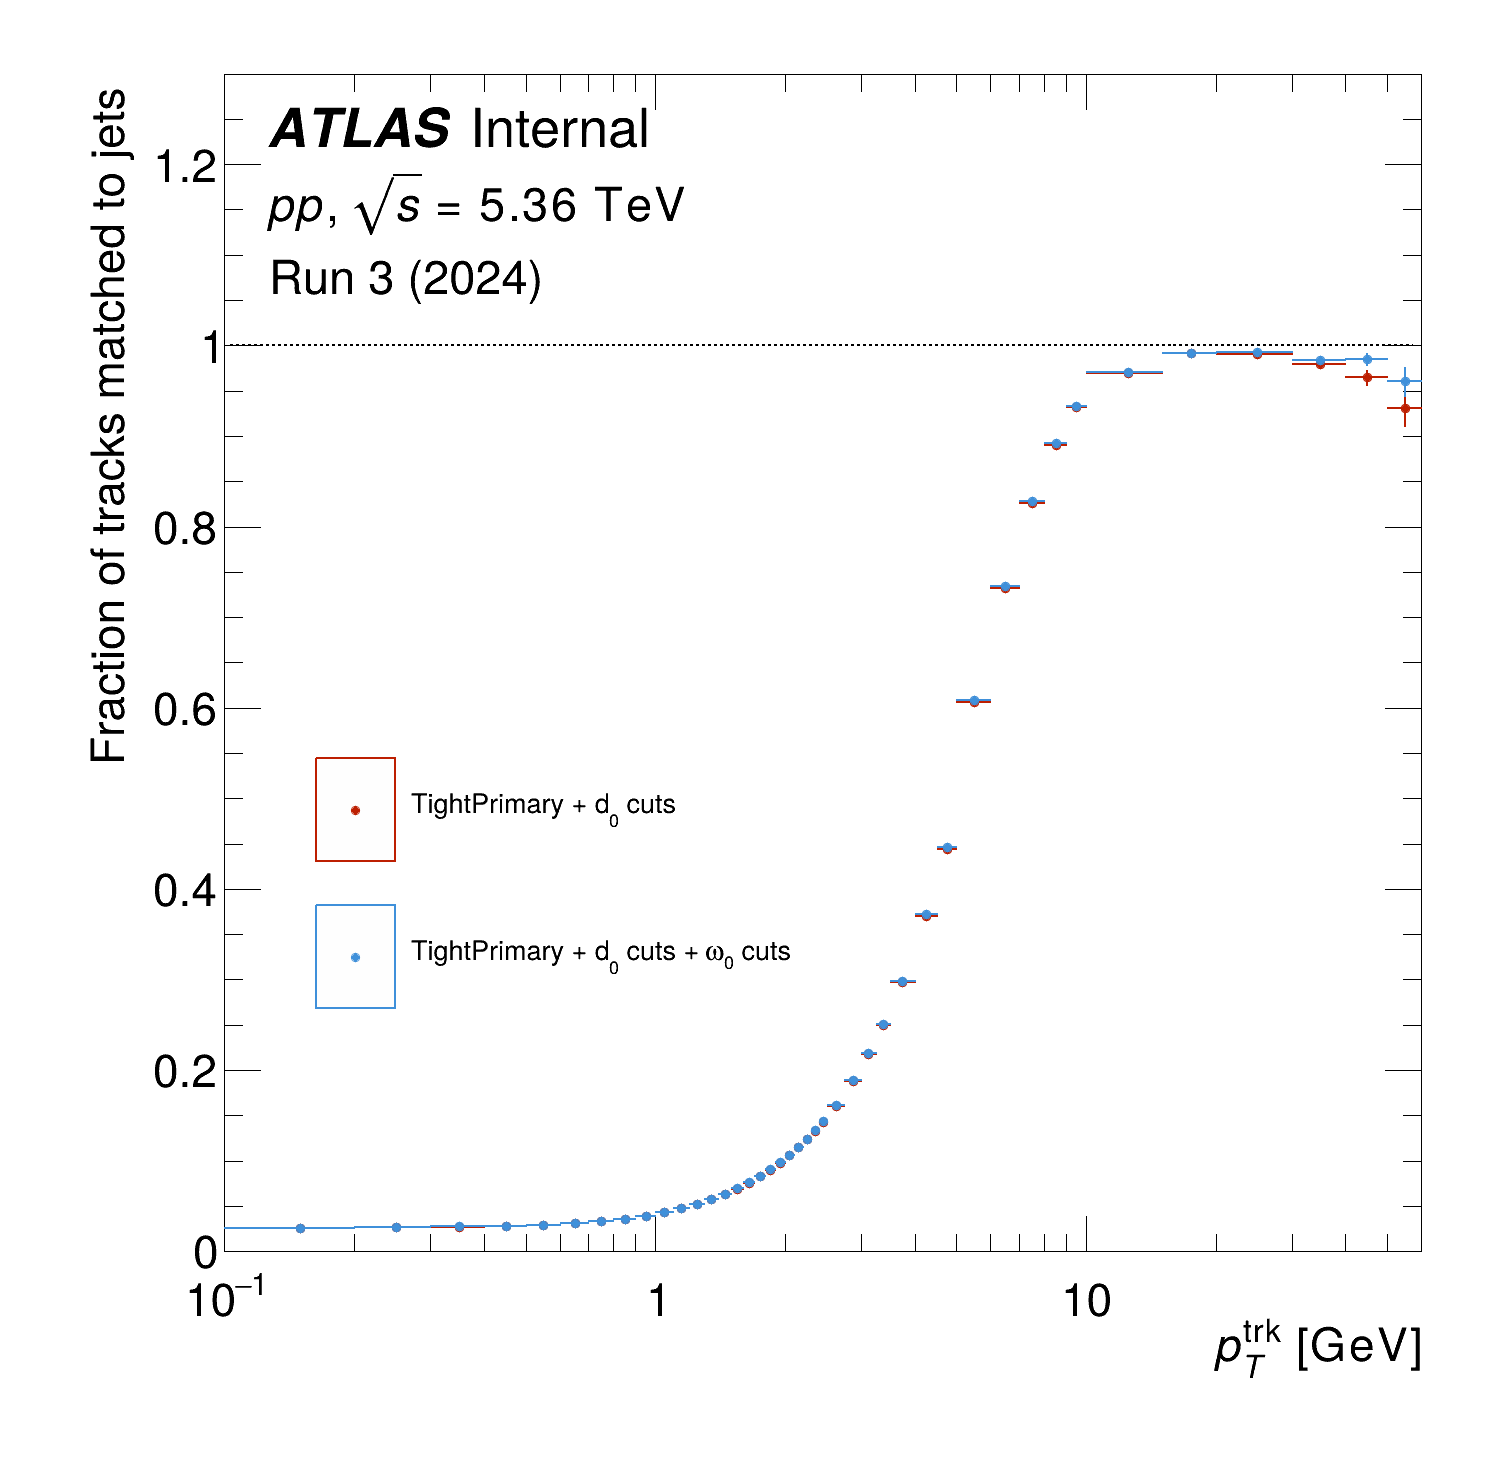
\includegraphics[width=0.55\linewidth]{images/trk_jetmatch0_.png}
    % 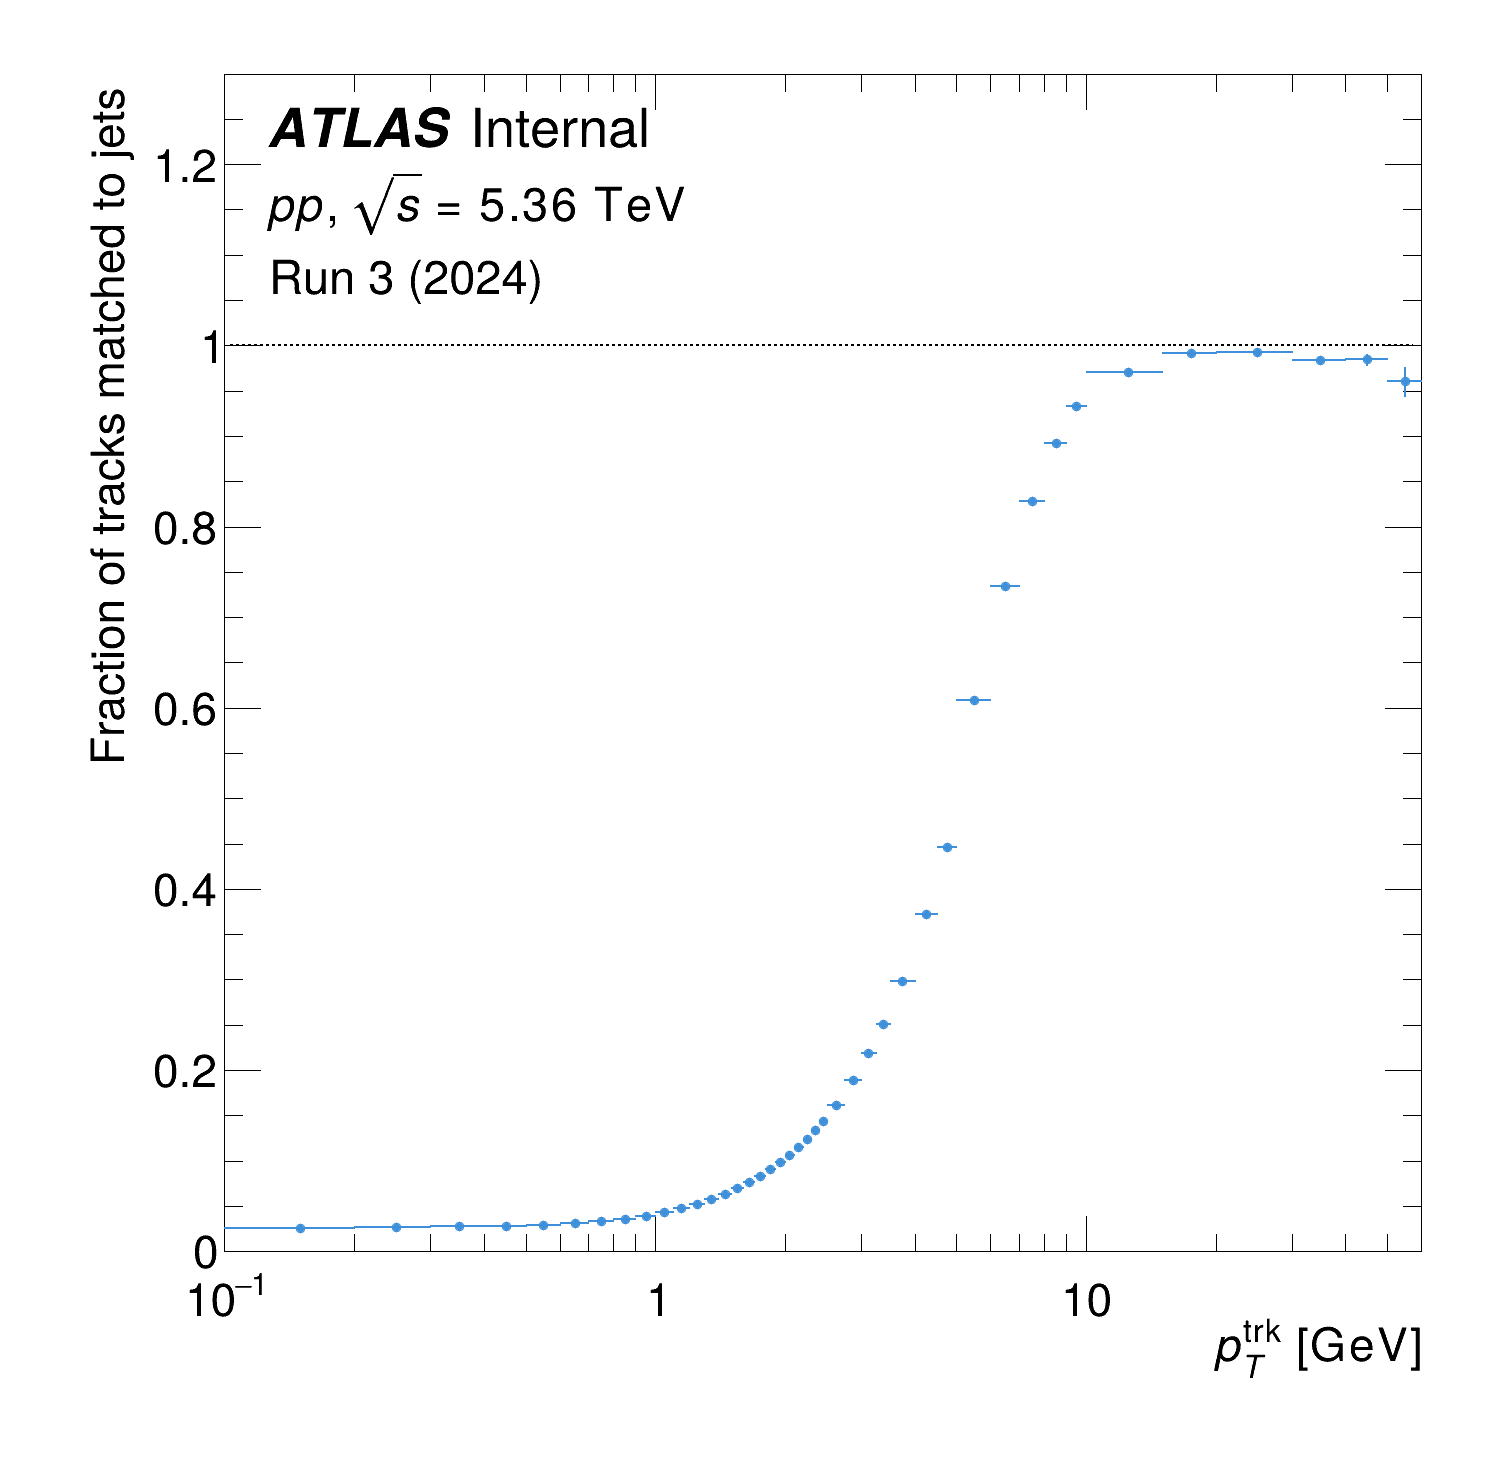
\includegraphics[width=0.49\linewidth]{images/trk_jetmatch1_.png}
    % \caption{Left: ''TightPrimary'' and $|d_0|<\qty{1.5}{\mm}$, $|d_0/\sigma_{d_0}| < 4$. Right: Additionally requiring $|\omega_0|<\qty{1.5}{\mm}$, $|\omega_0/\sigma_{\omega_0}| < 4$ and $|z_\text{vtx}|<\qty{150}{\mm}$}
    \caption{Track-to-jet association probability based on $dR<0.4$ cut for tracks selected using ''TightPrimary'' quality and $d_0$ cuts compared with additionaly using $\omega_0$ cuts}
    \label{fig:jetmatched_fractions}
\end{figure}

\section{Summary}
The final choice of track cuts used in the analysis is listed in Table~\ref{tab:tab_cuts}.
%{\red It'll be better to separate the d0 and z0 cuts into two lines, as we are unsure whether one shall apply both. If that is possible, move the percentiles of losses here. BTW, when you write that track, jet matching does not change the percentage; it's better that you only consider high-\pT tracks.}
\begin{table}[ht!]
  \caption{Track selection criteria in $\pprefSample$ data sample}%
  \label{tab:track_sel_pprefSample}
  \centering
  % \resizebox{\textwidth}{!}{
  \begin{tabular}{ll}
    \toprule
    Track quality    & \texttt{TightPrimary} \\
    Track-to-vertex matching criteria in $d_0$     & $|d_0| < \qty[parse-numbers=false]{1.5}{\mm}$ \\
    Track-to-vertex matching criteria in $\omega_0$     & $|\omega_0| < \qty[parse-numbers=false]{1.5}{\mm}$\\
    Significance cut on $d_0$                & $|d_0/\sigma_{d_0}| <4$ \\
    Significance cut on $\omega_0$                & $|\omega_0/\sigma_{\omega_0}| <4$ \\
    Associated vertex                & $|z_\text{vtx}| < \qty{150}{\mm}$ \\
    Track-to-jet association        & \(\mathrm{d}R < 0.4\) for $\pT>\qty{20}{\GeV}$ \\
    \bottomrule
    \label{tab:tab_cuts}
  \end{tabular}
  % }
\end{table}
The fraction of tracks selected after each cut (cutflow) in the high-$\mu$ sample is presented in Table~\ref{tab:cutflow_highmu}.
\begin{table}[h]
    \centering
    \caption{Cutflow on tracks in high-$\mu$ $\pprefSample$ sample}
    \begin{tabular}{c|c}
    Cut & Fraction after applying \\
    \hline
    Quality: ''Loose'' & $100\%$ \\
    Quality: ''TightPrimary'' & $84.9\%$ \\
    $|d_0| < 1.5$ mm & $78.5\%$ \\
    $|d_0/\sigma_{d_0}| < 4$ & $77.1\%$ \\
    $|\omega_0| < 1.5$ mm & $74.1\%$ \\
    $|\omega_0/\sigma_{\omega_0}| < 4$ & $72.1\%$ \\
    $|z_\text{vtx}| < 150$ mm & $71.2\%$ \\
    $dR<0.4$ \&\& $\pT>20$ GeV & $71.2\%$ \\
    \end{tabular}
    \label{tab:cutflow_highmu}
\end{table}
The same selection criteria will be applied in $\OOSample$ and $\NeNeSample$ samples. 

The resulting raw spectrum is presented in Figure~\ref {fig:trk_pt_cutflow}. See the performance of the cuts on different distributions in the appendix.
\begin{figure}[h]
    \centering
    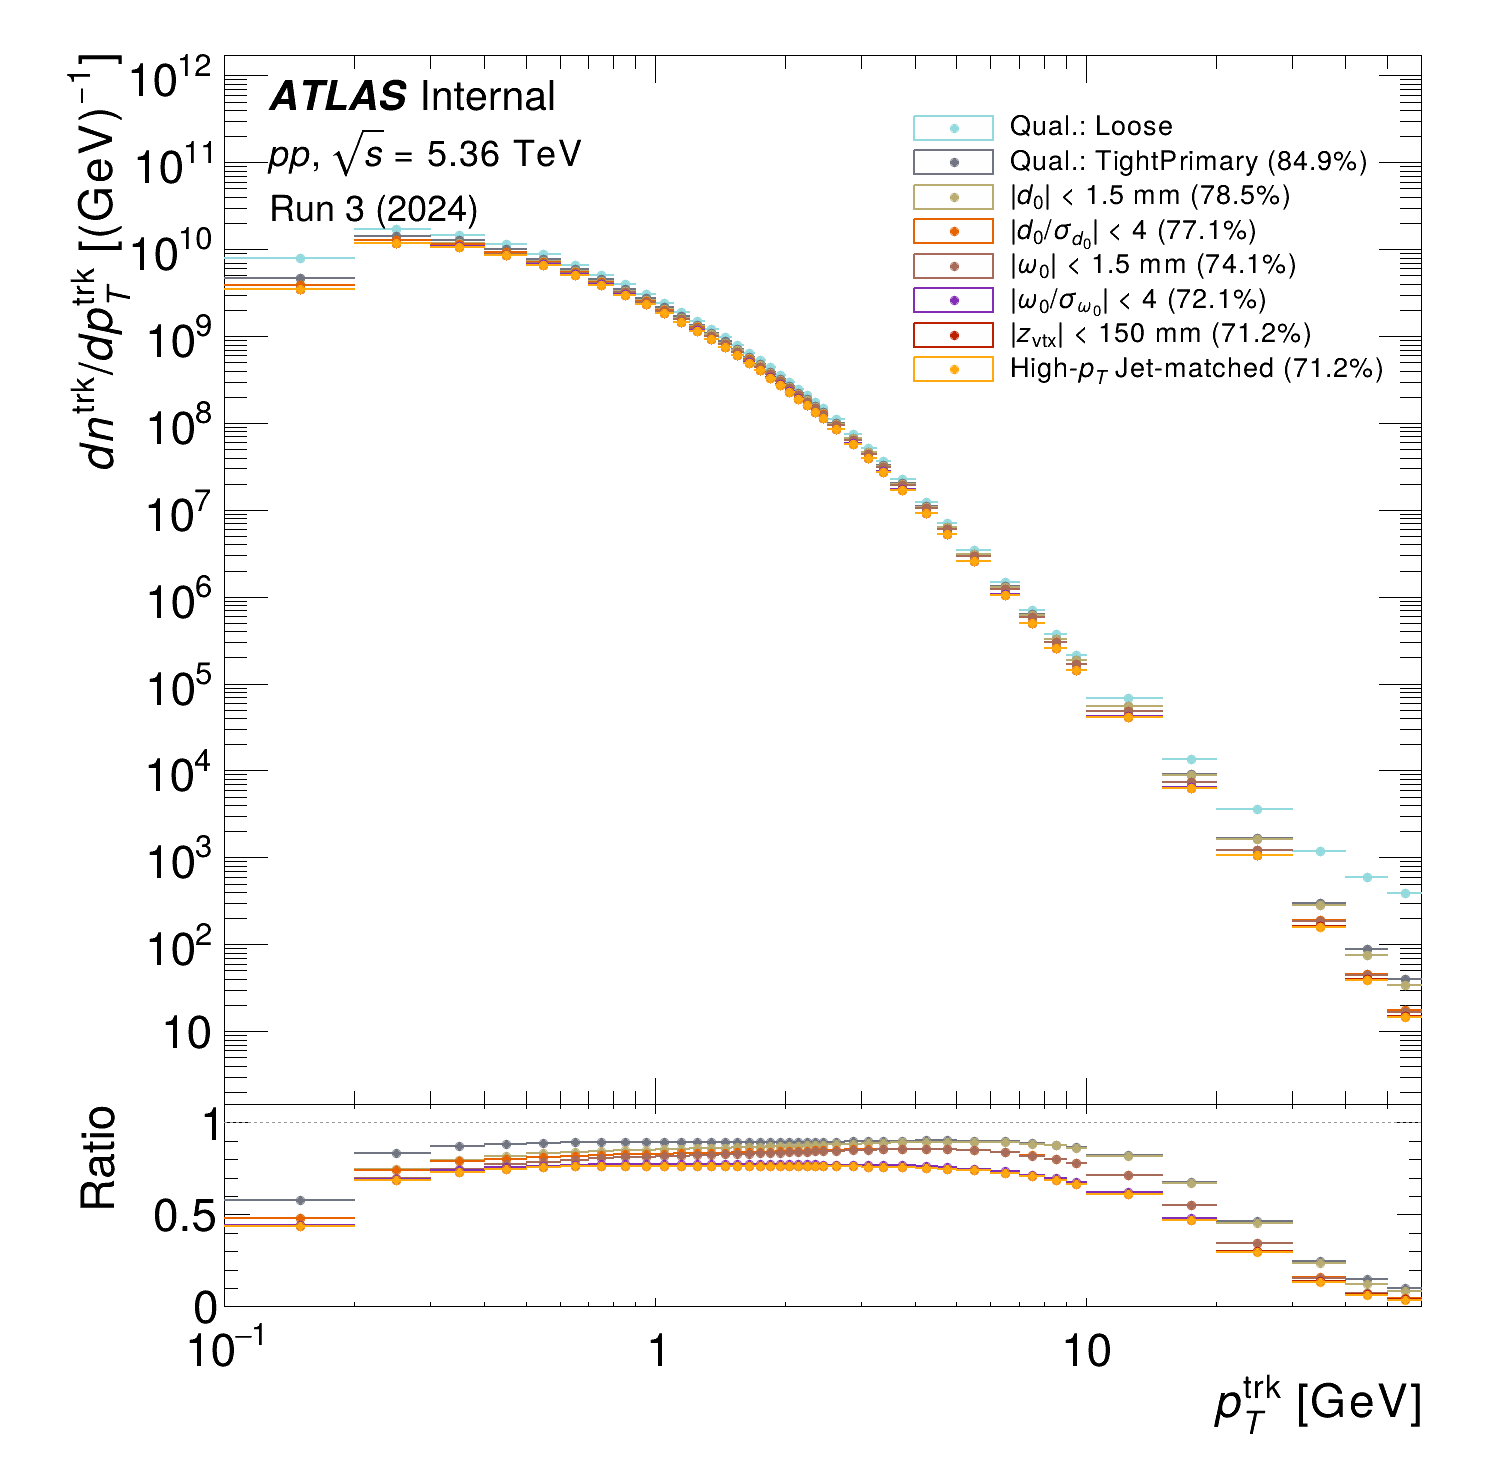
\includegraphics[width=0.49\textwidth]{images/trk_pt_cutflow_.png}
        \includegraphics[width=0.49\textwidth]{images/trk_Z0_cutflow_.png}
    \caption{Cutflow of \pT (left) and $z_0$ (right) distributions in \pp data. 
    %{\red Do you understand why jet matching cuts on z that much? }
    }
    \label{fig:trk_pt_cutflow}
\end{figure}



%\begin{figure}[h]
%    \centering
%    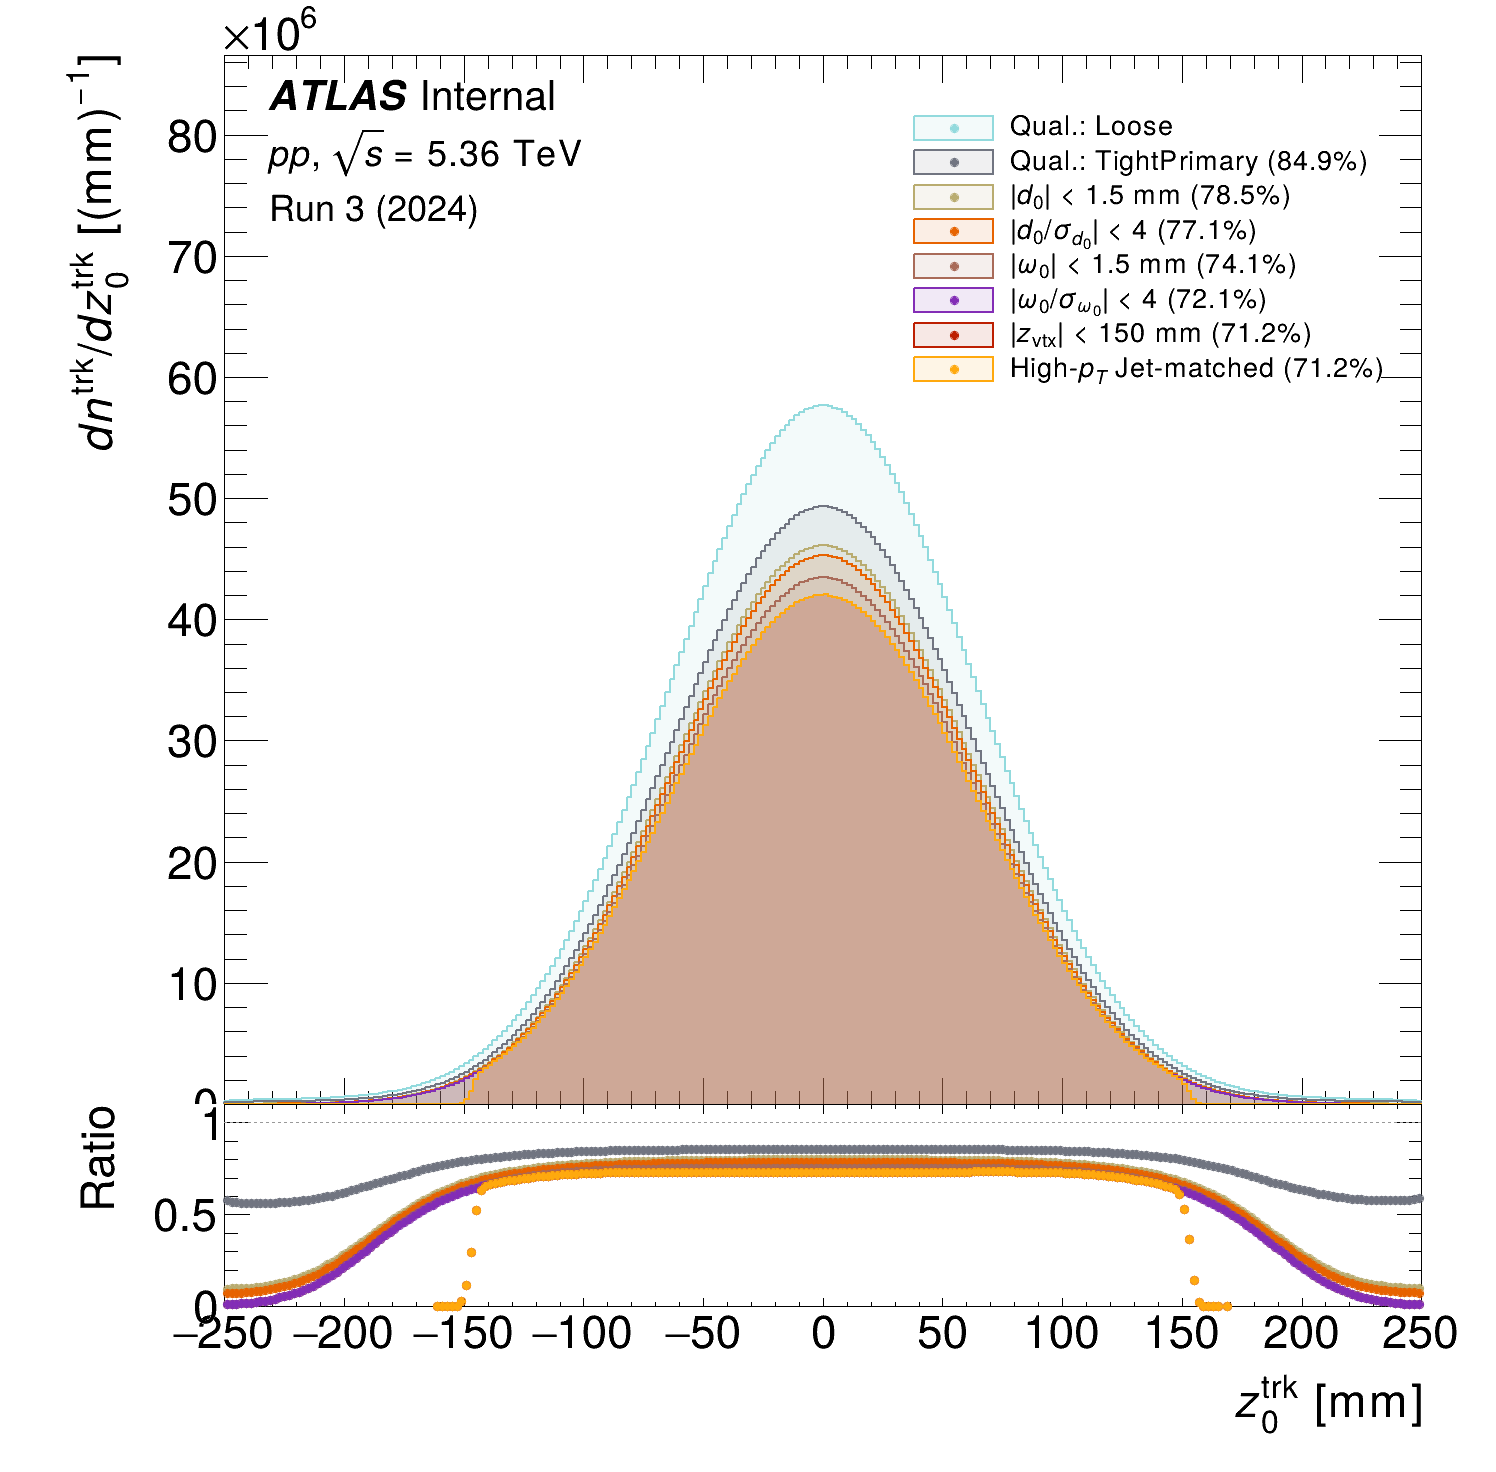
\includegraphics[width=0.5\linewidth]{images/trk_z0_cutflow_.png}
%    \caption{Selection cutflow as a function of $z_0$}
%    \label{fig:z0_cutflow}
%\end{figure}